\documentclass[conference]{IEEEtran}
\IEEEoverridecommandlockouts

\usepackage[utf8]{inputenc}
\usepackage[T1]{fontenc}
\usepackage{hyperref}
\usepackage{xargs}
\usepackage{listings}
\usepackage{minted}
\usepackage[outline]{contour}% http://ctan.org/pkg/contour
\usepackage{xspace}
\usepackage{amsmath}
\usepackage{color, colortbl}
\usepackage{booktabs}
\usepackage{pgfplots}
\usetikzlibrary{patterns}

\newif\iffinalversion
% Uncomment me for the final version.
\finalversiontrue

\iffinalversion
\usepackage[disable]{todonotes}

\renewcommand{\todo}[2]{}
\newcommandx{\wmnote}[1]{}
\newcommandx{\az}[1]{}
\newcommandx{\rz}[1]{}
\newcommandx{\lc}[1]{}
\newcommandx{\red}[1]{#1}
\else
\usepackage[textsize=scriptsize,textwidth=1.5in]{todonotes}

\addtolength{\marginparwidth}{1.2in}
\addtolength{\hoffset}{1.0in}
\addtolength{\paperwidth}{2.4in}

\newcommandx{\az}[2][1=]{\todo[linecolor=yellow,backgroundcolor=yellow!25,bordercolor=yellow,#1]{\textbf{Alex:} #2}}
\newcommandx{\wmnote}[2][1=]{\todo[linecolor=blue,backgroundcolor=blue!25,bordercolor=blue,#1]{\textbf{Billy:} #2}}
\newcommandx{\rz}[2][1=]{\todo[linecolor=green,backgroundcolor=green!25,bordercolor=green,#1]{\textbf{Ruizhe:} #2}}
\newcommandx{\lc}[2][1=]{\todo[linecolor=blue,backgroundcolor=blue!25,bordercolor=blue,#1]{\textbf{Lorenzo:} #2}}
\newcommand{\red}[1]{{\color{red} #1}}
\fi


\newcommand{\icode}[1]{{\texttt{#1}}}
\newcommand{\tool}{Polygeist\xspace}
\newcommand{\memref}{\icode{memref}\xspace}
\newcommand{\scop}{SCoP\xspace}
\newcommand{\polycc}{\icode{polycc}\xspace}

\tikzset{
  cfedge/.style={
    font=\itshape,
    draw=black,
    ->,
    >=stealth'
  },
  process/.style={
    draw,
    fill=orange!50,
    rectangle,
    minimum height=1.5em,
    minimum width=6em,
    align=center,
    font=\small,
  }
}

%\newcommand{\subheading}[1]{\vspace{0.3em}\noindent\textbf{\textit{#1:}}}
\newcommand{\subheading}[1]{\paragraph{#1}}
\newcommand{\midsepremove}{\aboverulesep = 0mm \belowrulesep = 0mm}
%\definecolor{orange3}{rgb}{0.808,0.361,0.000}
\definecolor{orange3}{rgb}{0.425,0.191,0.000}
\definecolor{scarletred3}{rgb}{0.643,0.000,0.000}
\definecolor{green3}{rgb}{0.000,0.405,0.000}
\definecolor{blue3}{rgb}{0.000,0.000,0.704}
\definecolor{aluminium1}{rgb}{0.933,0.933,0.925}
\definecolor{aluminium2}{rgb}{0.827,0.843,0.812}
\definecolor{aluminium3}{rgb}{0.729,0.741,0.714}
\definecolor{aluminium4}{rgb}{0.533,0.541,0.522}
\definecolor{aluminium5}{rgb}{0.333,0.341,0.325}
\definecolor{aluminium6}{rgb}{0.180,0.204,0.212}

\lstset{basicstyle=\ttfamily}

\lstdefinelanguage{llvm}{
	% see https://tex.stackexchange.com/questions/137237/listings-text-highlighting-based-on-prefix
    %moredelim=[s][\color{orange3}]{x}{>},
    alsoletter={\%,\#,!},
    keywordsprefix={\%},
    morekeywords={\%},
    keywordstyle=\color{orange3},
    commentstyle=\color{aluminium4},
    % this allows to color inside <memrefxf32> (i.e., f32).
    otherkeywords={index, f32, i32, f64, i8},
    keywords=[3]{index, f32, memref, i32, f64, i8, affine_map, affine_set, iter_args},
    keywordstyle=[3]\color{scarletred3},
    keywords=[4]{affine},
    keywordstyle=[4]\color{aluminium6},
    showstringspaces=false,
	breaklines=true,
    breakatwhitespace=true,
    morestring=[b]",
    stringstyle=\color{green3},
    moredelim=[s][\color{blue3}]{\#}{<},
    moredelim=[s][\color{scarletred3}]{!}{\ },
    morecomment=[l]{//},
}


%\title{Affine C in MLIR}
%\title{Polygeist: Revisiting Polyhedral Compilation in MLIR}
\title{Polygeist: Raising C to Polyhedral MLIR}
\author{
\IEEEauthorblockN{William S. Moses\IEEEauthorrefmark{1}}
\IEEEauthorblockA{
\textit{MIT CSAIL}\\
Cambridge, MA, USA\\
wmoses@mit.edu}
\and
\IEEEauthorblockN{Lorenzo Chelini\IEEEauthorrefmark{1}}
\IEEEauthorblockA{
\textit{TU Eindhoven}\\
Eindhoven, The Netherlands\\
l.chelini@tue.nl}
\and
\IEEEauthorblockN{Ruizhe Zhao\IEEEauthorrefmark{1}}
\IEEEauthorblockA{
\textit{Imperial College London}\\
London, UK\\
ruizhe.zhao15@imperial.ac.uk}
\and
\IEEEauthorblockN{Oleksandr Zinenko}
\IEEEauthorblockA{
\textit{Google Inc.}\\
Paris, France\\
zinenko@google.com}
\thanks{\IEEEauthorrefmark{1} Equal contribution.}
}

\newcommand{\toolseqspeedup}{$2.53\times$\xspace}
\newcommand{\pollyseqspeedup}{$1.41\times$\xspace}
\newcommand{\plutoseqspeedup}{$2.34\times$\xspace}

\newcommand{\toolparspeedup}{$9.47\times$\xspace}
\newcommand{\plutoparspeedup}{$7.54\times$\xspace}
\newcommand{\pollyparspeedup}{$3.26\times$\xspace}

\begin{document}

\maketitle

% IMPORTANT: no LaTex commands in the abstract!
\begin{abstract}
We present Polygeist, a new compilation flow that connects the MLIR compiler infrastructure to cutting edge polyhedral optimization tools. It consists of a C and C++ frontend capable of converting a broad range of existing codes into MLIR suitable for polyhedral transformation and a bi-directional conversion between MLIR and OpenScop exchange format. The Polygeist/MLIR intermediate representation featuring high-level (affine) loop constructs and n-D arrays embedded into a single static assignment (SSA) substrate enables an unprecedented combination of SSA-based and polyhedral optimizations. We illustrate this by proposing and implementing two extra transformations: statement splitting and reduction parallelization. Our evaluation demonstrates that Polygeist outperforms on average both an LLVM~IR-level optimizer (Polly) and a source-to-source state-of-the-art polyhedral compiler (Pluto) when exercised on the Polybench/C benchmark suite in sequential (2.53x vs 1.41x, 2.34x) and parallel mode (9.47x vs 3.26x, 7.54x) thanks to the new representation and transformations.
\end{abstract}


\section{Introduction}

Improving the efficiency of computation has always been one of the prime goals of computing.
Program performance can be improved significantly by reaping the benefits of parallelism, temporal and spatial locality, and other performance sources. Relevant program transformations are particularly tedious and challenging when targeting modern multicore CPUs and GPUs with deep memory hierarchies and parallelism, and are often performed automatically by optimizing compilers.

The polyhedral model enables precise analyses and a relatively easy specification of transformations (loop restructuring, automatic parallelization, etc.) that take advantage of hardware performance sources.  As a result, there is growing evidence that the polyhedral model is one of the best frameworks for efficient transformation of compute-intensive programs~\cite{tc,teckyl,mullapudi2015polymage},
% \az{I rephrased "machine learning programs" because we don't target ML programs specifically}
% agreed -wm
and for programming accelerator architectures~\cite{cerebras_chip,ppcg,tc_cim}. Consequently, the compiler community has focused on building tools that identify and optimize parts of the program that can be represented within the polyhedral model (commonly referred to as static-control parts, or \scop's). Such tools tend to\rz{Maybe just say there are two categories? And could we explicitly say one uses lower-level repr. and the other is rather higher-level (just to connect with the final paragraphs)?} fall into two categories.

% \az{I rewrote the two paragraphs below significantly. We are not contributing better \scop detection... (I understand there has been some work to implement that, but this is not exactly novel, sorry about that). Neither do we use hardware-specific things like vectorization.}
% \wmnote{agreed, I do wonder if there's anything more we can add as potential downsides of source style as its a bit bare}
% \az{We can, but we will not be using that later, so it can be used against us :)}
% fair point -wm, some good future work for sure :P

Compiler-based tools like Polly~\cite{grosser.ppl.2012} and Graphite~\cite{pop2006graphite} detect and transform {\scop}s in compiler intermediate representations (IRs). While this offers seamless integration with rest of the compiler, the lack of high-level structure and information hinders the tools' ability to perform analyses and transformations. This structure needs to be recovered from optimized IR, often imperfectly or at a significant cost~\cite{delinearization}. Moreover, common compiler optimizations such as LICM may interfere with the process~\cite{delicm}. Finally, low-level IRs often lack constructs for, e.g., parallelism or reductions, produced by the transformation, which makes the flow more complex.

\begin{figure}
\begin{center}
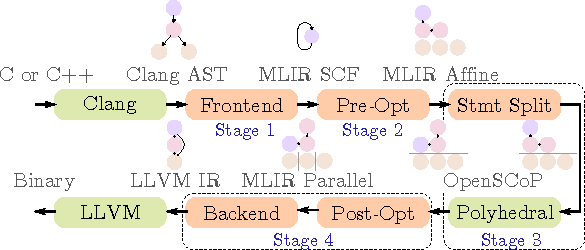
\includegraphics[scale=0.7]{images/mixed.pdf}
\caption{The \tool compilation flow consists of 4 stages. The frontend traverses Clang AST to emit MLIR SCF dialect (Section~\ref{sec:frontsub}), which is raised to the Affine dialect and pre-optimized (Section~\ref{sec:raising}). The IR is then processed by a polyhedral scheduler (Sections~\ref{sec:polyhedral_tools},\ref{sec:stmt_splitting}) before post-optimization and parallelization (Section~\ref{sec:opts}). Finally, it is translated to LLVM IR for further optimization and binary generation by LLVM.}
\label{fig:pipeline}
\end{center}
\end{figure}

Source-to-source compilers such as Pluto~\cite{Bondhugula2008Pluto}, \textsc{PoCC}~\cite{pocc} and \textsc{ppcg}~\cite{ppcg} operate directly on C or C++ code. While this can effectively leverage the high-level information from source code, the effectiveness of such tools is often reduced by the lack of enabling optimizations such as those converting hazardous memory loads into single-assignment virtual registers. Furthermore, the transformation results must be expressed in C, which is known to be complex~\cite{cloog,grosser2015polyhedral} and is also missing constructs for, e.g., reduction loops or register values not backed by memory storage.


This paper proposes and evaluates the benefits of a polyhedral compilation flow, \tool (Figure~\ref{fig:pipeline}), that can leverage both the high-level structure available in source code and the fine-grained control of compiler optimization provided by low-level IRs. It builds on the recent MLIR compiler infrastructure that allows the interplay of multiple abstraction levels within the same representation, during the same transformations~\cite{mlir}. Intermixable MLIR abstractions, or \emph{dialects}, include high-level constructs such as loops, parallel and reduction patterns; low-level representations fully covering LLVM IR~\cite{llvm}; and a polyhedral-inspired representation featuring loops and memory accesses annotated with affine expressions.
%However, there are presently no polyhedral scheduling transformations within MLIR.
% \rz{I feel that this line is a bit detached with the rest. Could we say things like ``Polygeist is the 1st tool that includes polyhedral scheduling transformations'' after this line.}
% \az{\tool is BY FAR not the first tool that includes polyhedral scheduling. I think we are better off without this claim.}
% \wmnote{basically was thinking of a way to say that mlir currently didn't schedule (to prevent the argument of oh you just used an existing thing, though perhaps thats not an actual concern), is this reasonable to say now or stil should be axed}
% \az{There \emph{are} polyhedral transformations in mlir, just no affine scheduling, and we are using some of those, i.e. parallelization. I wrote it... Uday has a preprint on optimizing matmul to BLIS level with MLIR. We are shooting ourselves by saying this.}
% \wmnote{Yeah I'm now convinced there's no good way to concisely describe what we want to say from this (i.e. a potential problem that is solved by creating polymer) without losing attention in all the details}
Moreover, by combining the best of source-level and IR-level tools in an end-to-end polyhedral flow, \tool preserves high-level information and leverages them to perform new or improved optimizations, such as statement splitting and loop-carried value detection, on a \emph{lower}-level abstraction as well as to influence downstream optimizations.

We make the following contributions:
\begin{itemize}
    \item a C and C++ frontend for MLIR that preserves high-level loop structure from the original source code;
    \item an end-to-end flow with raising to and lowering from the polyhedral model, leveraging our abstraction to perform more optimizations than both source- and IR-level tools, including reduction parallelization;
    \item an exploration of new transformation opportunities created by \tool, in particular, statement splitting;
    \item and an end-to-end comparison between \tool and state-of-the-art source- and IR-based tools (Pluto~\cite{Bondhugula2008Pluto} and Polly~\cite{grosser2015polyhedral}) along with optimization case studies.
\end{itemize}
%\az{Had to kill the result preview for space reasons}
%\tool achieves the largest speedups when evaluated on the Polybench suite~\cite{polybench} both serially and in parallel. 
\section{The MLIR Framework}
\subsection{Overview}
MLIR is an optimizing compiler infrastructure inspired by LLVM~\cite{llvm} with a focus on extensibility and modularity~\cite{mlir}. Its main novelty is the IR supporting a fully extensible set of instructions (called \emph{operations}) and types. Practically, MLIR combines SSA with nested regions, allowing one to express a range of concepts as first-class operations including machine instructions such as floating-point addition, structured control flow such as loops, hardware circuitry~\cite{circt}, and large machine learning graphs. Operations define the runtime semantics of a program and process immutable values. Compile-time information about values is expressed in \emph{types}, and information about operations is expressed in \emph{attributes}. Operations can have attached regions, which in turn contain (basic) blocks of further operations. The generic syntax, accepted by all operations, illustrates the structure of MLIR in Figure~\ref{fig:mlir_syntax}. Additionally, MLIR supports user-defined custom syntax.

\begin{figure}
{
\scriptsize
\begin{lstlisting}[language=llvm,escapeinside=@@, mathescape=true]
%result = "dialect.operation"(%operand, %operand)
          {attribute = #dialect<"value">} ({
// Inside a nested region.
^basic_block(%block_argument: !dialect.type):
  "another.operation"() : () -> ()
}) : (!dialect.type) -> !dialect.result_type
\end{lstlisting}
}
\caption{Generic MLIR syntax for an operation with two operands, one result, one attribute and a single-block region.}
\label{fig:mlir_syntax}
\end{figure}

Attributes, operations, and types are organized in \emph{dialects}, which can be thought of as modular libraries. MLIR provides a handful of dialects that define common operations such as modules, functions, loops, memory or arithmetic instructions, and ubiquitous types such as integers and floats. We discuss the dialects relevant to \tool in the following sections.

\subsection{Affine and MemRef Dialects}\label{sec:affine_memref}

The \emph{Affine} dialect~\cite{mlir_affine} aims at representing \scop's with explicit polyhedral-friendly loop and conditional constructs.
The core of its representation is the following classification of value categories:
\begin{itemize}
    \item \emph{Symbols}---integer values that are known to be loop-invariant but unknown at compile-time, also referred to as program \emph{parameters} in polyhedral literature, typically array dimensions or function arguments. In MLIR, symbols are values defined in the top-level region of an operation with ``affine scope'' semantics, e.g., functions; or array dimensions, constants, and affine map (see below) application results regardless of their definition point.
    \item \emph{Dimensions}---are an extension of symbols that also accepts induction variables of affine loops.
    \item \emph{Non-affine}---any other values.
\end{itemize}
Symbols and dimensions have \icode{index} type, which is a platform-specific integer that fits a pointer (\icode{intptr\_t} in C).

MLIR provides two attributes relevant for the Affine dialect:
\begin{itemize}
\item
\emph{Affine maps} are multi-dimensional (quasi-)linear functions that map a list of dimension and symbol arguments to a list of results.
For example, $(d_0, d_1, d_2, s_0) \rightarrow (d_0 + d_1, s_0 \cdot d_2)$ is a two-dimensional quasi-affine map, which can be expressed
in MLIR as \icode{affine\_map<(d0,d1,d2)[s0] -> (d0+d1, s0*d2)>}.
%The affine map construct does \emph{not} require its arguments to have the symbol and dimension category, only \emph{some} operations in the affine dialect do.
Dimensions (in parentheses on the left) and symbols (in brackets on the left) are separated to allow quasi-linear expressions: symbols are treated as constants, which can therefore be multiplied with dimensions, whereas a product of two dimensions is invalid.
\item
\emph{Integer sets} are collections of integer tuples constrained by conjunctions of (quasi-)linear expressions.
For example, a ``triangular'' set $\{(d_0, d_1) : 0 \leq d_0 < s_0 \land 0 \leq d_1 \leq d_0\}$ is represented as
\icode{affine\_set<(d0,d1)[s0]: (d0 >= 0, s0-d0-1 >= 0, d1 >= 0, d0-d1 >= 0)>}.
\end{itemize}


The Affine dialect makes use of the concepts above to define a set of operations.
An \icode{affine.for} is a ``for'' loop with loop-invariant lower and upper bounds expressed as affine maps with a constant step.
An \icode{affine.parallel} is a ``multifor'' loop nest, iterations of which may be executed concurrently.
Both kinds of loops support reductions via loop-carried values as well as max(min) expression lower(upper) bounds.
%The region is a single block that corresponds to the body of the loop and takes the induction variable as a loop argument.
An \icode{affine.if} is a conditional construct, with an optional \icode{else} region, and a condition defined as inclusion of the given values into an integer set.
Finally, \icode{affine.load} and \icode{affine.store} express memory accesses where the address computation is expressed as an affine map.

\begin{figure}
{
\scriptsize
\begin{lstlisting}[language=llvm, escapeinside=@@, mathescape=true]
%c0 = constant 0 : index
%0 = memref.dim %A, %c0 : memref<?xf32>
%1 = memref.dim %B, %c0 : memref<?xf32>
affine.for %i = 0 to affine_map<()[s0] -> (s0)>()[%0] {
  affine.for %j = 0 to affine_map<()[s0] -> (s0)>()[%1] {
    %2 = affine.load %A[%i] : memref<?xf32>
    %3 = affine.load %B[%j] : memref<?xf32>
    %4 = mulf %2, %3 : f32
    %5 = affine.load %C[%i + %j] : memref<?xf32>
    %6 = addf %4, %5 : f32
    affine.store %6, %C[%i + %j] : memref<?xf32>
  }
}
\end{lstlisting}
}
\vspace{-.5cm}
\caption{Polynomial multiplication in MLIR using Affine and Standard dialects.}
\label{fig:polynomial}
\end{figure}

Figure~\ref{fig:polynomial} illustrates the Affine dialect for a polynomial multiplication, \icode{C[i+j] += A[i] * B[j]}.
This simple example highlights the fact that MLIR supports, and encourages, IRs from different dialects to be used together.

% \begin{figure}
%     \centering
%     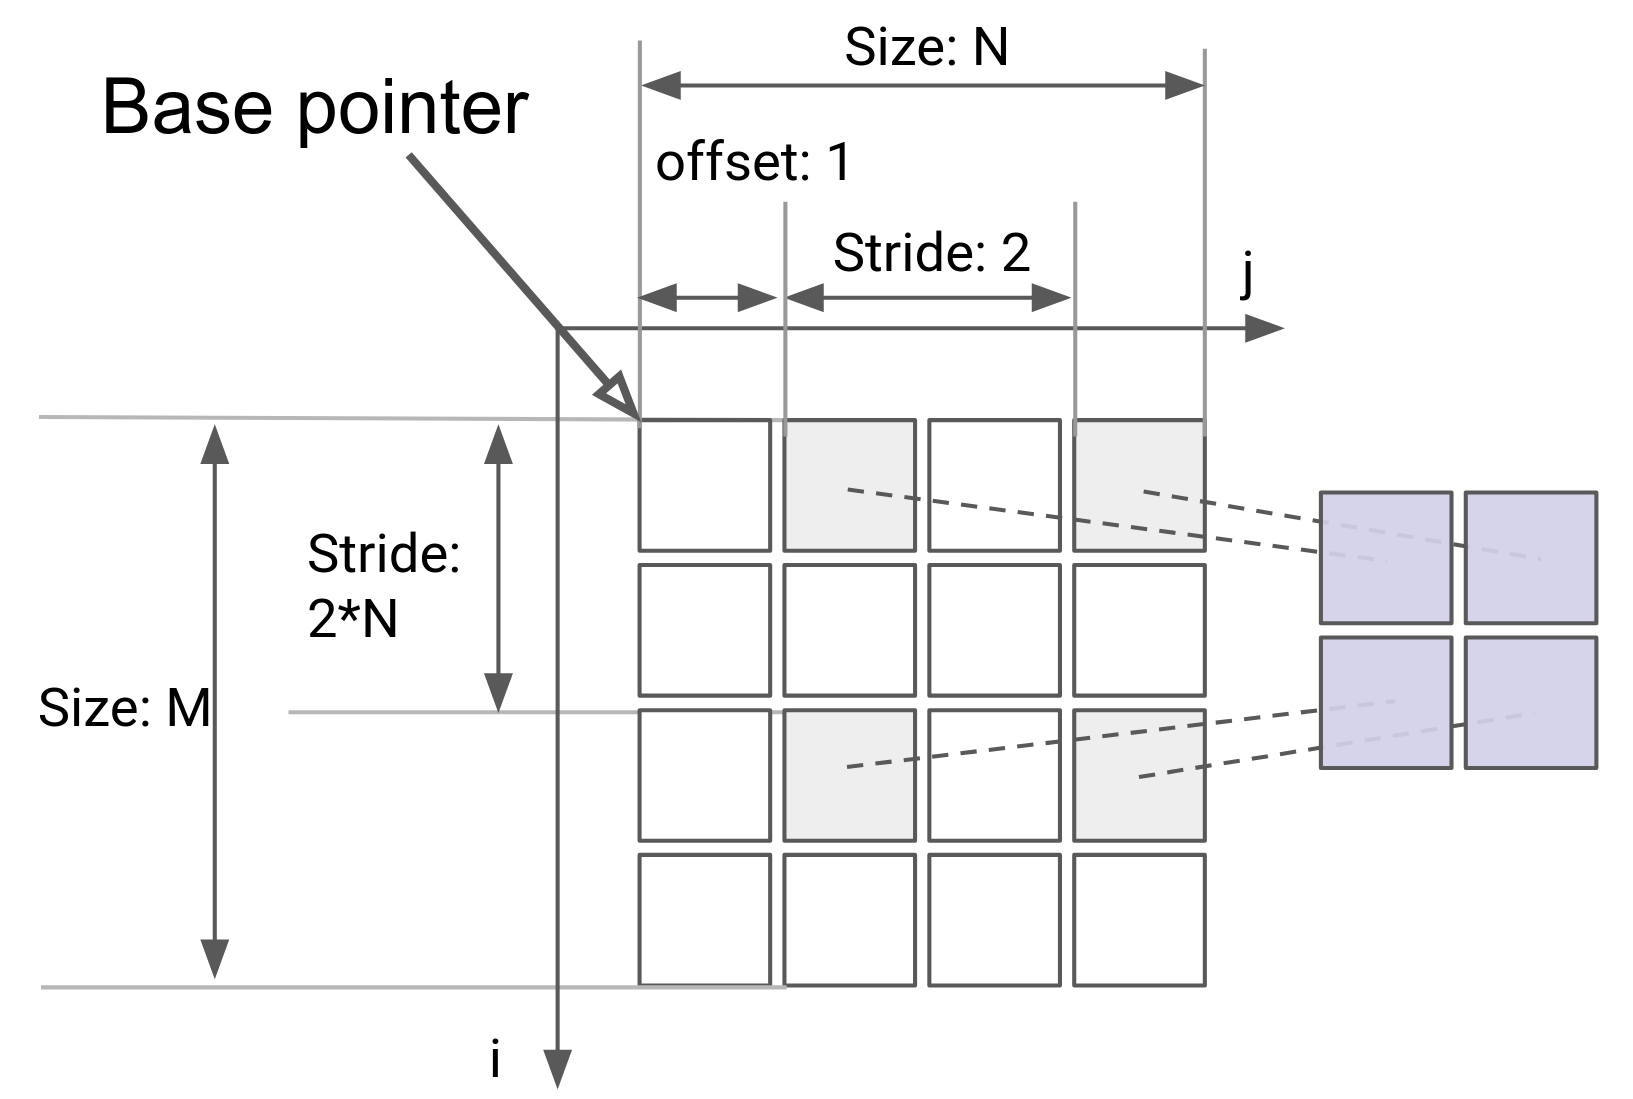
\includegraphics[width=0.7\columnwidth]{images/memref.png}
%     \vspace{-.5cm}
%     \caption{MLIR supports multi-dimensional memory references indexed with affine maps.}
%     \label{fig:memref}
% \end{figure}

A core MLIR type---\memref, which stands for \textbf{mem}ory \textbf{ref}erence---and the corresponding \emph{\memref dialect} are also featured in Figure~\ref{fig:polynomial}. The \memref type describes a structured multi-index pointer into memory, e.g., \icode{memref<?xf32>} denotes a 1-d array of floating-point elements; and the \emph{\memref dialect} provides memory and type manipulation operations, e.g., \icode{memref.dim} retrieves the dimensionality of a \memref object.
\memref does not allow internal aliasing, i.e., different subscripts always point to different addresses.
This effectively defines away the delinearization problem that hinders the application of polyhedral techniques at the LLVM IR level~\cite{delinearization}.
Throughout this paper, we only consider {\memref}s with the default \emph{layout} that corresponds to contiguous row-major storage compatible with C ABI (Application Binary Interface). In practice, {\memref}s support arbitrary layouts expressible as affine maps, but these are not necessary in \tool context.

%By default, {\memref}s are expected to have a \emph{strided} format similar to the one used for tensors in machine learning %frameworks.
%A strided \memref is described by its \emph{rank}, \emph{offset} from the base pointer, a list of \emph{sizes} and a list of \emph{strides}.
%The latter indicates the number of elements one needs to skip to obtain the next element along a dimension.
%Strides can thus express various layouts.
%For example, an $M \times N$ \memref with strides $N, 1$ is row-major, with strides $1, M$ is column-major, while the strides $2N$ and $2$ combined with $\mathrm{offset}=1$ define a layout accessing odd columns in even lines as illustrated in Figure~\ref{fig:memref}.
%In general, the list of indices is transformed into the linear address as 
%$A = \mathrm{base} + \mathrm{offset} + \sum_i \mathrm{stride}_i \cdot \mathrm{index}_i.$
%One can observe that, for a fixed rank, this can be expressed using an affine map by treating offset and strides as symbols:
%\icode{affine\_map<(i0,i1)[A,off,s0,s1] -> (A + off + s0*i0 + s1*i1)>}.
%This is intentional and makes {\memref}s compatible with affine transformations.


\subsection{Other Relevant Core Dialects}
MLIR  provides several dozen dialects.
Out of those, only a handful are relevant for our discussion:
\begin{itemize}
\item
The \emph{Structured Control Flow} (\icode{scf}) dialect defines the control flow operations such as loops and conditionals that are not constrained by affine categorization rules.
For example, the \icode{scf.for} loop accepts any integer value as loop bounds, which are not necessarily affine expressions.
\item
The \emph{Standard} (\icode{std}) dialect contains common operations such as integer and float arithmetic, which is used as a common lowering point from higher-level dialects before fanning out into multiple target dialects and can be seen as a generalization of LLVM IR~\cite{llvm}.
\item
The \emph{LLVM} dialect directly maps from LLVM IR instructions and types to MLIR, primarily to simplify the translation between them.
\item
The \emph{OpenMP} dialect provides a dialect- and platform-agnostic representation of OpenMP directives such as ``parallel'' and ``workshare loop'', which can be used to transform OpenMP constructs or emit LLVM IR that interacts with the OpenMP runtime.
\item
The \emph{Math} dialect groups together mathematical operations on integer and floating type beyond simple arithmetic, e.g., \icode{math.pow} or \icode{math.sqrt}.
\end{itemize}
\section{An (Affine) MLIR Compilation Pipeline}

The \tool pipeline consists of 4 components (Figure~\ref{fig:pipeline}):
\begin{enumerate}
    %\item a frontend that allows entering MLIR at the SCF + Affine loops level from C or C++ code (Section~\ref{sec:frontsub});
    \item a frontend that allows entering MLIR at the SCF loops level from C or C++ code (Section~\ref{sec:frontsub});
    %\item a preprocessing step within MLIR that raises the non-loop operations to the Affine dialect (Section~\ref{sec:raising});
    \item a preprocessing step within MLIR that raises to the Affine dialect (Section~\ref{sec:raising});
    \item a polyhedral scheduler of the Affine parts of the program \textit{via} a round-trip to and from OpenSCoP (Section~\ref{sec:polyhedral_tools}) and running Pluto transformations, controlled by the new statement splitting heuristic (Section~\ref{sec:stmt_splitting});
    \item a backend that runs postprocessing MLIR optimizations (section~\ref{sec:opts}) and final lowering to an executable.
\end{enumerate}

\subsection{Frontend}
\label{sec:frontsub}
\tool builds off the Clang compiler to emit MLIR, directly analyzing Clang's AST. \tool thus avoids reimplementing parsing and language-level semantic analysis and handles modern C and C++ features. As is typical for compiler frontends, \tool creates a recursive symbol table data structure to look up the correct variable for a given scope. \tool lazily registers all global variables and functions found in the AST to its symbol table before generating any code. \tool then traverses the call graph from a given entry function (\texttt{main} by default), creating and defining MLIR functions as necessary.
%\wmnote{AST from entry function is incorrect, the call graph is the correct term. The reason is that we basically create a queue funcctions we need to emit starting from main, hence call graph. just AST implies we emit all which is not true (as we lazily emit).}
\subheading{Control Flow \& High Level Information}

In contrast to traditional compiler pipelines, targeting a branch-based IR, \tool leverages the high-level MLIR operations such as \texttt{scf.while} (a looping construct) and \texttt{scf.if} (a conditional construct) within the SCF dialect to preserve the control flow structure of the source code. C-level \icode{continue} and \icode{break} constructs are handled by introducing signal
variables and checking them before each operation that follows original constructs. Furthermore, within a \texttt{\#pragma scop}, \tool assumes that the program is affine and uses an \texttt{affine.for} to represent loops directly.
%\az{I removed the \icode{continue} example. While nice, it is useless for the benchmarks we discuss. Replaced that with one sentence that says we can handle break/continue.}\wmnote{Yeah that's fine. The one thing that we may want to use is another example of how we may have to add special handling (that thus especially needs additional preprocessing optimizations such as mem2reg/if merging}

% Preserving this in comment if parts needed in future
% Some operators within MLIR may not directly correspond to C and C++-level semantics. For example, high-level loop operators within MLIR do not permit the use of the \texttt{continue} construct. When this abstraction mismatch occurs, \tool emits wrapper code that enables the correct behavior. For example, \texttt{continue} is modeled by creating a new boolean that represents whether a continue statement has been executed and wrapping all loop statements within a conditional that checks whether one hit a \texttt{continue} (Figure \ref{fig:continue}).

% \begin{figure}
%     \centering
% \begin{tabular}{c}
% \begin{minipage}[t]{0.95\linewidth}
% \begin{minted}[fontsize=\small, escapeinside=||]{cpp}
% for (int i=0; i<N; ++i) {
%     A(i);
%     if (B(i))
%         continue;
%     C(i);
% }
% \end{minted}
% \end{minipage}\\
% \begin{minipage}[t]{0.95\linewidth}
% \begin{minted}[fontsize=\small, escapeinside=@@]{cpp}
%              @$\big\Downarrow$@
% bool seenContinue;
% for (int i=0; i<N; ++i) {
%     seenContinue = false;
%     if (!seenContinue)
%         A(i);
%     if (!seenContinue)
%         if (B(i))
%             seenContinue = true;
%     if (!seenContinue)
%         C(i);
% }
% \end{minted}
% \end{minipage} 
% \end{tabular}
%     \caption{Top: a C program that contains a continue statement. Bottom: a rewrite of the code above that eliminates the continue statement while preserving the original program's semantics. \tool performs such a transformation when lowering to MLIR (rather than emitting C) as MLIR's high-level loop constructs do not permit \texttt{continue}.}
%     \label{fig:continue}
% \end{figure}

\begin{figure}
  \centering
  \resizebox{\columnwidth}{!}{%
  {\tt
  \begin{tabular}{lll}
  \toprule
  {\rm\bf C type} & {\rm\bf LLVM IR type} & {\rm\bf MLIR type} \\
  \midrule
  int & i32 (on machine X) & i32 (on machine X) \\
  intNN\_t & iNN & iNN \\
  uintNN\_t & iNN & uiNN \\
  float & float & f32 \\
  double & double & f64 \\
  ty * & ty * & memref<?\,x\,ty> \\
  ty \& & ty * & memref<1\,x\,ty> \\
  ty ** & ty ** & memref<memref<?\,x\,ty>\ \!\!\!> \\
  ty[N][M] & [N x [M x ty]]* & memref<N\,x\,M\,x\,ty> \\
  \bottomrule
  \end{tabular}
  }
  }
  \caption{Type correspondence between C, LLVM IR and MLIR types.}
  \label{fig:types}
\end{figure}

\subheading{Types \& \tool ABI}
While emitting operations, \tool must decide how to represent C or C++ types within MLIR. For primitive types such as \texttt{int} or \texttt{float}, \tool emits an MLIR variant of that type with the same width as would be used within LLVM/Clang. This allows \tool to keep the same ABI as code compiled by a normal C or C++ compiler when calling a function with only primitive types. On the other hand, for pointer, reference and array types, \tool uses \memref type (Figure~\ref{fig:types}). This allows \tool to preserve more of the structure available within the original program (e.g., multi-dimensional arrays) and enables interaction with MLIR's high-level memory operations.

This diverges from the C ABI for any functions with pointer arguments and wouldn't interface correctly with C functions. \tool addresses this by providing an attribute for function arguments and allocations to use a C-compatible pointer type rather than \memref, applied by default to external functions such as \texttt{strcmp} and \texttt{scanf}. When calling a pointer-ABI function with a \texttt{memref}-ABI argument, \tool generates wrapper code that recovers the C ABI-compatible pointer from \memref and ensures the correct result.
% When a function with C-compatible ABI is called with a \memref argument, \tool extracts the raw pointer and passes it to the function call, which is made possible by only considering contiguous row-major {\memref}s.
%\wmnote{The extract row-major is not accurate. For functions like scanf we actually make a temporary llvm pointer buffer, then load result of buffer and store into memref}
Figure~\ref{fig:abi} shows an example demonstrating how the \tool and C ABI may interact for a small program.

%To ease programmers' burden from having to specify an %ABI attribute on code not compiled by \tool, we %automatically apply the pointer ABI attribute to C %library functions and \texttt{main}. %Figure~\ref{fig:abi} shows an example demonstrating how %the \tool and C ABI may interact for a small program.

When allocating and deallocating memory, this difference in ABI becomes significant. This is because allocating several bytes of an array with \icode{malloc} then casting to a \memref will not result in legal code (as \memref itself may not be implemented with a raw pointer). Thus, \tool identifies calls to allocation and deallocation functions and replaces them with legal equivalents for \memref. 

Functions and global variables are emitted using the same name used by the C or C++ ABI. This ensures that all external values are loaded correctly, and multi-versioned functions (such as those generated by \texttt{C++} templates or overloading) have distinct names and definitions.

\subheading{Instruction Generation}
For most instructions, \tool directly emits an MLIR operation corresponding to the equivalent C operation (\icode{addi} for integer add, \icode{call} for function call, etc.).  For some special instructions such as a call to \texttt{pow}, \tool chooses to emit a specific MLIR operation in the Math dialect, instead of a call to an external function (defined in libm). This permits such instructions to be better analyzed and optimized within MLIR.

Operations that involve memory or pointer arithmetic require additional handling. MLIR does not have a generic pointer arithmetic instruction; instead, it requires that \texttt{load} and \texttt{store} operations contain all of the indices being looked up. This presents issues for operations that perform pointer arithmetic. To remedy this, we introduce a temporary \texttt{subindex} operation for \memref's keeps track of the additional address offsets. A subsequent optimization pass within \tool, forwards the offsets in a \texttt{subindex} to any \texttt{load} or \texttt{store} which uses them.
% \az{I changed this to say \icode{subindex} is a temp operation, it doesn't matter if we proposed it or not IMO.}
% sgtm

\subheading{Local Variables}
Local variables are handled by allocating a \memref on stack at the top of a function. This permits the desired semantics of C or C++ to be implemented with relative ease. However, as many local variables and arguments contain \memref types, this immediately results in a \memref of a \memref---a hindrance for most MLIR optimizations as it is illegal outside of \tool. As a remedy, we implement a heavyweight memory-to-register (mem2reg) transformation pass that eliminates unnecessary loads, stores, and allocations within MLIR constructs. Empirically this eliminates all {\memref}s of \memref in the Polybench suite.


\subsection{Raising to Affine}\label{sec:raising}

The translation from C or C++ to MLIR directly preserves high-level information about loop structure and n-D arrays, but does not generate other Affine operations. \tool subsequently raises memory, conditional, and looping operations into their Affine dialect counterparts if it can prove them to be legal affine operations. If the corresponding frontend code was enclosed within \texttt{\#pragma scop}, \tool assumes it is always legal to raise all operations within that region without additional checks.\footnote{All kernels within Polybench are successfully raised to Affine with or without the use of \texttt{\#pragma scop}.} Any operations which are not proven or assumed to be affine remain untouched. We perform simplifications on affine maps to remove loops with zero or one iteration and drop branches of a conditional with a condition known at compile time.

\subheading{Memory operations and loop bounds}
To convert an operation, \tool replaces its bound and subscript operands with identity affine maps (\icode{affine\_map<() [s0]->(s0)>[\%bound]}). It then folds the operations computing the map operands, e.g., \icode{addi}, \icode{muli}, into the map itself. Values that are transitively derived from loop induction variables become map dimensions and other values become symbols. For example, \icode{affine\_map<\ ()[s0]->(s0)>[\%bound]} with \icode{\%bound = addi \%N, \%i}, where \icode{\%i} is an induction variable, is folded into \icode{affine\_map<(d0)[s0] ->(s0 + d0)>(\%i)[\%N]}. The process terminates when no operations can be folded or when Affine value categorization rules are satisfied.

\subheading{Conditionals}
Conditional operations are emitted by the frontend for two input code patterns: \icode{if} conditions and ternary expressions. The condition is transformed by introducing an integer set and by folding the operands into it similarly to the affine maps, with in addition \icode{and} operations separating set constraints and \icode{not} operations inverting them (\icode{affine.if} only accepts $\geq 0$ and $=0$ constraints). \tool processes nested conditionals with C-style short-circuit semantics, in which the subsequent conditions are checked within the body of the preceding conditionals, by hoisting conditions outside the outermost conditional when legal and replacing them with a boolean operation or a \icode{select}. This is always legal within \icode{\#pragma scop}.

Conditionals emitted for ternary expressions often involve memory loads in their regions, which prevent hoisting due to side effects. We reuse our mem2reg pass to replace those to equivalent earlier loads when possible to enable hoisting. Empirically, this is sufficient to process all ternary expressions in the Polybench/C suite~\cite{polybench}. Otherwise, ternary expressions would need to be packed into a single statement by the downstream polyhedral pass.

\begin{figure}
    \centering
    {\scriptsize
\begin{lstlisting}[language=c]
void setArray(int N, double val, double* array) {...}
int main(int argc, char** argv) {
  ...
  cmp = strcmp(str1, str2)
  ...
  double array[10];
  setArray(10, 42.0, array)
}
\end{lstlisting}}
\vspace{-0.5cm}
$\Downarrow$
{\scriptsize
\begin{lstlisting}[language=llvm, escapeinside=&&]
func @setArray(%N: i32, %val: f64,
               %array: memref<?xf64>) {
  %0 = &\color{black}{\tt index\_cast}& %N : i32 to index
  affine.for %i = 0 to %0 {
    affine.store %val, %array[%i] : memref<?xf64>
  }
  return
}

func @main(%argc: i32,
           %argv: !llvm.ptr<ptr<i8>>) -> i32 {
  ...
  %cmp = llvm.call @strcmp(%str1, %str2) :
           (!llvm.ptr<i8>, !llvm.ptr<i8>) -> !llvm.i32
  ...
  %array = memref.alloca() : memref<10xf64>
  %arraycst = memref.cast %array : memref<10xf64> to 
    memref<?xf64>
  %val = constant 42.0 : f64
  call @setArray(%N, %val, %arraycst) :
           (i32, f64, memref<?xf64>) -> ()
}
\end{lstlisting}}
    \caption{Example demonstrating \tool ABI. For functions expected to be compiled with \tool such as \icode{setArray}, pointer arguments are replaced with \memref's. For functions that require external calling conventions (such as \icode{main}/\icode{strcmp}), \tool falls back to emitting \icode{llvm.ptr} and generates conversion code.}
    \label{fig:abi}
\end{figure}
\subsection{Connecting MLIR to Polyhedral Tools}
\label{sec:polyhedral_tools}

Regions of the input program expressed using MLIR Affine dialect are amenable to the polyhedral model. Existing tools, however, cannot directly consume MLIR. We chose to implement a bi-directional conversion to and from OpenScop~\cite{openscop}, an exchange format readily consumable by numerous polyhedral tools, including Pluto~\cite{Bondhugula2008Pluto}, and further convertible to \icode{isl}~\cite{isl} representation. This allows \tool to seamlessly connect with tools created in polyhedral compilation research without having to amend those tools to support MLIR.

Most polyhedral tools are designed to operate on C or \textsc{Fortran} inputs build around \emph{statements}, which do not have a direct equivalent in MLIR. Therefore, we design a mechanism to create statement-like structure from chains of MLIR operations. We further demonstrate that this gives \tool an ability to favorably affect the behavior of the polyhedral scheduler by controlling statement granularity (Section~\ref{sec:stmt_splitting}).

\subheading{Simple Statement Formation}\label{sec:stmt_formation}
Observing that C statements amenable to the polyhedral model are (mostly) variable assignments, we can derive a mechanism to identify statements from chains of MLIR operations. A \icode{store} into memory is the last operation of the statement.
The backward slice of this operation, i.e., the operations transitively computing its operands, belong to the statement. The slice extension stops at operations producing a value categorized as affine dimension or symbol, directly usable in affine expressions. Such values are loop induction variables or loop-invariant constants.

Some operations may end up in multiple statements if the value is used more than once. However, we need the mapping between operations and statements to be bidirectional in order to emit MLIR after the scheduler has restructured the program without considering SSA value visibility rules. If an operation with multiple uses is side effect free, \tool simply duplicates it. For operations whose duplication is illegal, \tool stores their results in stack-allocated \memref's and replaces all further uses with memory loads. Figure~\ref{fig:scratchpad} illustrates the transformation for value \icode{\%0} used in operation \icode{\%20}. This creates a new statement.

\subheading{Region-Spanning Dependencies}

In some cases, a statement may consist of MLIR operations across different (nested) loops, e.g., a load from memory into an SSA register happens in an outer loop while it is used in inner loops. The location of such a statement in the loop hierarchy is unclear. More importantly, it cannot be communicated to the polyhedral scheduler. \tool resolves this by storing the value in a stack-allocated \icode{memref} in the defining region and loading it back in the user regions. Figure~\ref{fig:scratchpad} illustrates this transformation for value \icode{\%0} used in operation \icode{\%10}. Similarly to the basic case, this creates a new statement in the outer loop that can be scheduled independently.

This approach can be seen as a reg2mem conversion, the inverse of mem2reg performed in the frontend. It only applies to a subset of values, and may be undone after polyhedral scheduling has completed. Furthermore, to decrease the number of dependencies and memory footprint, \tool performs a simple value analysis and avoids creating stack-allocated buffers if the same value is already available in another memory location and can be read from there.
\wmnote{for now just removed the nuanced mem2reg description (in comment here).}
% Even though this can be thought as a pass which ``undoes''
% .\lc{I would remove this last sentence.} 

%While it is possible to instead make frontend mem2reg less aggressive, it would lead to more statements and associated dependencies that negatively affect the performance of the polyhedral scheduler.\wmnote{this is confusing}

\begin{figure}
\centering
{\scriptsize
\begin{lstlisting}[language=llvm, escapeinside=**, mathescape=true]
affine.for %i = ...
  %0 = affine.load %A[%i]
  affine.store %other, %A[%i] // motion-barrier
  affine.for %j = ... {
    %1 = affine.load %B[%j]
    %10 = mulf %0, %1 : f64   // use-1
    store %10, %res[%i, %j]
  %20 = addf %0, %0 : f64     // use-2
\end{lstlisting}}
$\Downarrow$
{\scriptsize
\begin{lstlisting}[language=llvm, escapeinside=**, mathescape=true]
%tmp = memref.alloca() : memref<1xf64>
affine.for %i = ...
  %0 = affine.load %A[%i]
  affine.store %0, %tmp[0]    // store to scratchpad
  affine.store %other, %A[%i] // motion-barrier
  affine.for %j = ...
    %1 = affine.load %B[%j]
    %2 = affine.load %tmp[0]  // load back for use-1
    %10 = mulf %2, %1 : f64   // use-1 (%2 instead of %0)
    affine.store %10, %res[%i, %j]
  %19 = affine.load %tmp[0]   // load back for use-2
  %20 = addf %19, %19 : f64   // use-2 (%19 instead of %0)
  // ...
\end{lstlisting}
}
\caption{\tool breaks region-spanning use-def chains and handles multi-use values by introducing scratchpad storage when operation duplication is illegal. In absence of \icode{motion-barrier} statement, the \icode{\%0} load would be duplicated and sunk. Pseudo-MLIR with types and braces omitted for brevity.}
\label{fig:scratchpad}
\end{figure}

\begin{figure}
{\scriptsize
\begin{lstlisting}[language=llvm, escapeinside=**, mathescape=true]
func @S1(%A: memref<?xf64>, %tmp: memref<1xf64>,
         %i: index)
  %0 = affine.load %A[%i]
  affine.store %0, %tmp[0]   // store to scratchpad

func @S2(%A: memref<?xf64>, %other: f64, %i: index)
  affine.store %other, %A[%i]

func @S3(%B: memref<?x?xf64>, %tmp: memref<1xf64>,
         %res: memref<?x?xf64>, %i: index, %j: index)
  %1 = affine.load %B[%k, %j]
  %2 = affine.load %tmp[0]   // load back for use-1
  %10 = mulf %2, %1 : f64    // use-1
  affine.store %10, %res[%i, %j]

func @S4(%tmp: memref<1xf64>, ...)
  %19 = affine.load %tmp[0]  // load back for use-2
  %20 = addf %19, %19 : f64  // use-2
  // ...

%tmp = memref.alloca() : memref<1xf64>
affine.for %i = ...
  call @S1(%A, %tmp, %i)
  call @S2(%A, %other, %i)
  affine.for %j = ...
    call @S3(%B, %tmp, %res, %i, %j)
  call @S4(%tmp)
\end{lstlisting}
}
\caption{Outlining makes polyhedral ``statements'' visible in code from Fig.~\ref{fig:scratchpad}.}
\label{fig:outlining}
\end{figure}

\subheading{\scop Formation}

To define a \scop, we outline individual statements into functions so that they can be represented as opaque calls with known memory footprints, similarly to Pencil~\cite{pencil}.
This process also makes the inter-statement SSA dependencies clear. These dependencies exist between calls that \emph{use} the same SSA value, but there are no values defined by these calls. We lift all local stack allocations and place them at the entry block of the surrounding function in order to keep them visible after loop restructuring. Figure~\ref{fig:outlining} demonstrates the resulting IR.

The remaining components of the polyhedral representation are derived as follows:
the domain of the statement is defined to be the iteration space of its enclosing loops, constrained by their respective lower and upper bounds, and intersected with any ``if'' conditions. This process leverages the fact that MLIR expresses bounds and conditions directly as affine constructs.
The access relations for each statement are obtained as unions of affine maps of the \icode{affine.load} (read) and \icode{affine.store} (must-write) operations, with RHS of the relation annotated by an ``array'' that corresponds to the SSA value of the accessed \memref.
Initial schedules are assigned using the $(2d+1)$ formalism, with odd dimensions representing the lexical order of loops in the input program and even dimensions being equal to loop induction variables.
Affine constructs in OpenScop are represented as lists of linear equality ($=0$) or inequality ($\geq 0$) coefficients, which matches exactly the internal representation in MLIR, making the conversion straightforward.


\subheading{Code Generation Back to MLIR}

The Pluto scheduler produces new schedules in OpenScop as a result. Generating loop structure back from affine schedules is a solved, albeit daunting, problem~\cite{cloog,grosser2015polyhedral}. \tool relies on CLooG~\cite{cloog} to generate an initial loop-level AST, which it then converts to Affine dialect loops and conditionals. There is no need to simplify affine expressions at code generation since MLIR accepts them directly and can simplify them at a later stage. Statements are introduced as function calls with rewritten operands and then inlined.

\subsection{Controlling Statement Granularity}\label{sec:stmt_splitting}

Recall that \tool reconstructs ``statements'' from sequences of primitive operations (Section~\ref{sec:polyhedral_tools}). We initially designed an approach that recovers the statement structure similar to that in the C input, but this is not a requirement. Instead, statements can be formed from any subsets of MLIR operations as long as they can be organized into loops and sorted topologically (i.e., there are no use-def cycles between statements). To expose the dependencies between such statements to the affine scheduler, we reuse the idea of going through scratchpad memory: each statement writes the values required by other statements to dedicated memory locations, and the following statements read from those. The scratchpads are subject to partial array expansion~\cite{array_expansion} to minimize their effect on the affine scheduler as single-element scratchpad arrays create artificial scalar dependencies.
%\az{discuss the potential of considering such dependencies differently in the scheduler or using live-range reordering, but this is out of scope because requires to change the scheduler.}
This change in \emph{statement granularity} gives the affine scheduler unprecedented flexibility allowing it to chose different schedules for different \emph{parts} of the same C statement.

\begin{figure}
  %\centering
  {\scriptsize
  \begin{lstlisting}[language=c]
for(i=0; i<NI; i++)
  for(j=0; j<NJ; j++)
    for(k=0; k<NK; k++)
S:    A[i][j]+=f(B[k][i],C[k][j]);
  \end{lstlisting}
  }\vspace{-0.5em}\par
  \hspace{0.25\linewidth}$\Downarrow$\vspace{0.5em}\par
  \begin{tabular}{@{\hspace{-\parindent}}l@{\hspace{-1em}$\Rightarrow$}l}
  {\scriptsize
  \begin{lstlisting}[language=c]
for(i=0; i<NI; i++)
  for(j=0; j<NJ; j++)
    double M[NK];
    for(k=0; k<NK; k++)
S:    M[k]=f(B[k][i],C[k][j]);
T:    A[i][j] += M[k];
  \end{lstlisting}
  }
  &
  {\scriptsize
  \begin{lstlisting}[language=c]
double M[NK];
for(k=0; k<NK; k++)
  for(i=0; i<NI; i++)
    for(j=0; j<NJ; j++)
 S:   M[k]=f(B[k][i],C[k][j]);
 T:   A[i][j] += M[k];
  \end{lstlisting}
  }
  \end{tabular}
  \caption{Splitting a nested reduction statement (top) into a fully parallel compute statement and a trivial reduction statement (bottom left) makes Pluto generate different schedules (bottom right). Further scratchpad array expansion may enable loop fission and give scheduler even more liberty.}
  \label{fig:splitting_example}
\end{figure}

Consider, for example, the statement \icode{S} in Figure~\ref{fig:splitting_example}(top) surrounded by three loops iterating over \icode{i}, \icode{j} and \icode{k}. Such contraction patterns are common in computational programs (this particular example can be found in the \icode{correlation} benchmark with \icode{B}$\equiv$\icode{C}, see Section~\ref{sec:splitcase}). The loop order that best exploits the locality is (\icode{k}, \icode{i}, \icode{j}), which results in temporal locality for reads from \icode{B} (the value is reused in all iterations of the now-innermost \icode{j} loop) and in spatial locality for reads from \icode{C} (consecutive values are read by consecutive iterations, increasing the likelihood of L1 cache hits). Yet, Pluto never proposes such an order because of a reduction dependency along the \icode{k} dimension due to repeated read/write access to \icode{A[i][j]} as Pluto tends to pick loops with fewer dependencies as outermost.
%\az{practically, in minimizes the upper bound of the dependence distance, which is never 0 along k because of the reduction, but can be zero along i and j here. Not sure if we want to go into such details.}
While the dependency itself is inevitable, it can be moved into a separate statement \icode{T} in Figure~\ref{fig:splitting_example}(bottom left). This approach provides scheduler with more freedom of choice for the first statement at a lesser memory cost than expanding the entire \icode{A} array. It also factors out the reduction into a ``canonical'' statement that is easier to process for the downstream passes, e.g., vectorization.

Implementing this transformation at the C level would require manipulating C AST and reasoning about C (or even C++) semantics. This is typically out of reach for source-to-source polyhedral optimizers such as Pluto that treat statements as black boxes. While it is possible to implement this transformation at the LLVM IR level, e.g., in Polly, where statements are also reconstructed and injection of temporary allocations is easy, the heuristic driving the transformation is based on the loop structure and multi-dimensional access patterns which are difficult to recover at such a low level~\cite{delinearization}.

The space of potential splittings is huge---each MLIR operation can potentially become a statement. Therefore, we devise a heuristic to address the contraction cases similar to Figure~\ref{fig:splitting_example}. Reduction statement splitting applies to statements:
\begin{itemize}
  \item surrounded by at least 3 loops;
  \item with LHS$\neq$RHS, and using all loops but the innermost;
  \item with two or more different access patterns on the RHS.
\end{itemize}
This covers statements that could have locality improved by a different loop order and with low risk of undesired fission.
This heuristic merely serves as an illustration of the kind of new transformations \tool can enable.
\subsection{Post-Transformations and Backend}\label{sec:opts}

\tool allows one to operate on both quasi-syntactic and SSA level, enabling analyses and optimizations that are extremely difficult, if not impossible, to perform at either level in isolation. In addition to statement splitting, we propose two techniques that demonstrate the potential of \tool.% for designing such optimizations.

\subheading{Transforming Loops with Carried Values (Reductions)}

\tool leverages MLIR's first-class support for loop-carried values to detect, express and transform reduction-like loops. This support does not require source code annotations, unlike source-level tools~\cite{reduction_drawing} that use annotations to enable detection, nor complex modifications for parallel code emission, unlike Polly~\cite{polly_reduction}, which suffers from LLVM missing first-class parallel constructs. We do not modify the polyhedral scheduler either, relying on post-processing for reduction parallelization, including outermost parallel reduction loops.

The overall approach follows the definition proposed in~\cite{10.1145/318789.318810} with adaptations to MLIR's region-based IR, and is illustrated in Figure~\ref{fig:red}. \tool identifies memory locations modified on each iteration, i.e. \icode{load}/\icode{store} pairs with loop-invariant subscripts and no interleaving aliasing \icode{store}s, by scanning the single-block body of the loop. These are transformed into \emph{loop-carried values} or secondary induction variables, with the \icode{load}/\icode{store} pair lifted out of the loop and repurposed for reading the initial and storing the final value. Loop-carried values may be updated by a chain of side effect-free operations in the loop body. If this chain is known to be associative and commutative, the loop is a \emph{reduction}. Loop-carried values are detected even in absence of reduction-compatible operations. Loops with such values contribute to mem2reg, decreasing memory footprint, but are not subject to parallelization.

\begin{figure}
\centering
\begin{tabular}{l@{$\Rightarrow$}l}
{\scriptsize
\begin{lstlisting}[language=llvm]
affine.for %i = ... {
  // Reduction into r1[0]
  %1 = affine.load %r1[0]
  %5 = addi %1, %2
  affine.store %5, %r1[0]
  // Loop-dependent load
  %10 = affine.load %r2[%i]
  %15 = addi %10, %2
  // Inteleaving store
  %20 = affine.load %r2[0]
  affine.store %21, %r2[0]
  %25 = addi %20, %2
  // May have side effects
  %30 = affine.load %r3[0]
  call @f(%30, %2)
}
\end{lstlisting}
}&{
\scriptsize
\begin{lstlisting}[language=llvm]
%init = affine.load %r1[0]
%red = affine.for %i = ...
 iter_args(%arg = %init) {
  // Reduction accumulation
  %5 = addi %arg, %2
  // Loop-dependent load
  %10 = affine.load %r2[%i]
  %15 = addi %10, %2
  // Inteleaving store
  %20 = affine.load %r2[0]
  affine.store %21, %r2[0]
  %25 = addi %20, %2
  // May have side effects
  %30 = affine.load %r3[0]
  call @f(%30, %2)
  // Yield accumulated 
  affine.yield %5
}
affine.store %red, %r1[0]
\end{lstlisting}
}
\end{tabular}
\caption{\tool detects memory locations accessed in all loop iterations, e.g. reduction accumulators such as \icode{\%r1[0]} and transforms them to loop-carried values (secondary induction variables), except when computed with side-effects, interleaved stores or  by non-associative/commutative operations.}
\label{fig:red}
\end{figure}


%\caption{\tool detect and manipulate reductions at the Affine level. Output of the reduction pass for a simple sequential array sum computation.}


%\az{I'm not sure Fig.~\ref{fig:red} brings something interesting to the paper.}

\subheading{Late Parallelization}\label{sec:parallelization}
Rather than relying on the dependence distance information obtained by the affine scheduler, \tool performs a separate polyhedral analysis to detect loop parallelism in the generated code. The analysis itself is a classical polyhedral dependence analysis~\cite{feautrier1991dataflow,eisenbeis1992general} implemented on top of MLIR region structure. Performing it after SSA-based optimizations, in particular mem2reg and reduction detection, allows parallelizing more loops. In particular, reduction loops and loops with variables whose value is only relevant within a single iteration similar to live-range reordering~\cite{verdoolaege2016live} but without expensive additional polyhedral analyses (live-range of an SSA value defined in a loop never extends beyond the loop).

%\subheading{Final Code Generation}
%After all subsequent MLIR optimizations, \tool emits LLVM IR suitable for the Clang/LLVM compiler. This can be used to emit a final binary or link to existing \tool or C ABI-compiled program.
%\lc{This takes space and not to important imo}

% generates affine MLIR by parsing Clang's Abstract Syntax Tree and progressively proving raising  Figure~\ref{fig:pipeline} shows an overview of \tool. Starting from a code fragment expressed using C or C++, \tool traverses the Clang AST and for each visited node emits the corresponding MLIR SCF or Standard dialect construct. 
% At SCF level, \tool exposes a raising pass which allows lifting Standard load, store, as well as SCF ``for'' loops and ``if'' conditions to the Affine dialect. At the Affine level, code is optimized and lowered back to SCF, which in turn, gets lowered to LLVM IR for code generation. Finally, \icode{Clang} takes LLVM IR and emits binary code, to be executed on the target platform.
\section{Evaluation}
Our evaluation has two goals. 1) We want to demonstrate that the code produced by \tool without additional optimization does not have any inexplicable performance differences than a state-of-the-art compiler like Clang. 2) We explore how \tool's internal representation can support a mix of affine and SSA-based transformation in the same compilation flow, and evaluate the potential benefits compared to existing source and compiler-based polyhedral tools.

%Our goal is twofold: First, we want to demonstrate that the code generated by \tool is on-par with the code generated by a state-of-the-art compiler like Clang (Section~\ref{sub:frontend}). Second, we wish to demonstrate the feasibility of utilizing existing polyhedral flows, especially research compilers, to process MLIR (Section~\ref{sub:polymer}).
%We are \emph{not} interested in using MLIR to produce better-optimized code than polyhedral flows.

\subsection{Experimental Setup}

We ran our experiments on an AWS \icode{c5.metal} instance with hyper-threading and Turbo Boost disabled. %(Table~\ref{table:arch}).
The system is Ubuntu 20.04 running on a dual-socket Intel Xeon Platinum 8275CL CPU at 3.0~GHz with 24 cores each, with 0.75, 35, 35.75~MB L1, L2, L3 cache per socket, respectively, and 256~GB RAM.
We ran all 30 benchmarks from PolyBench~\cite{polybench}, using the ``EXTRALARGE'' dataset. Pluto is unable to extract \scop from the \icode{adi} benchmark. We ran a total of 5 trials for each benchmark, taking the execution time reported by PolyBench; the median result is taken unless stated otherwise. Every measurement or result reported in the following sections refers to double-precision data. All experiments were run on cores 1-8, which ensured that all threads were on the same socket and did not potentially conflict with processes scheduled on core 0.

% \begin{table}
% \caption{Hardware setup.}
% \label{table:arch}
% \centering
% \resizebox{\columnwidth}{!}{%
% \begin{tabular}{lllll}
%     \toprule
%     \footnotesize{CPU} & 
%     \footnotesize{Clock rate} & 
%     \footnotesize{OS} & 
%     \footnotesize{RAM (GB)} & 
%     \footnotesize{L1/L2/L3 (MB)} \\ \midrule

%     \footnotesize{Intel Xeon Platinum 8275CL} & 
%     \footnotesize{3.0 GHz} & 
%     \footnotesize{Ubuntu 20.04} & 
%     \footnotesize{256} &
%     \footnotesize{1.5, 48, 71.5} \\ \bottomrule
% \end{tabular}
% }
% \end{table}

In all cases, we use two-stage compilation: (i) using \icode{clang} at \icode{-O3} excluding unrolling and vectorization; or \tool to emit LLVM IR from C; (ii) using \icode{clang} at \icode{-O3} to emit the final binary. As several optimizations are not idempotent, a second round of optimization can potentially significantly boost (and rarely, hinder) performance. This is why we chose to only perform vectorization and unrolling at the last optimization stage. Since \tool applies some optimizations at the MLIR level (e.g., mem2reg), we compare against the two-stage compilation pipeline as a more fair baseline (\textsc{Clang}). We also evaluate a single-stage compilation to assess the effect of the two-stage flow (\textsc{ClangSing}).

\subsection{Baseline Performance}
\label{sub:frontend}
\tool must generate code with runtime \emph{as close as possible} to that of existing compilation flows to establish a solid baseline. In other words, \tool should \emph{not introduce overhead nor speedup} unless explicitly instructed otherwise, to allow for measuring the effects of additional optimizations. We evaluate this by comparing the runtime of programs produced by \tool with those produced by Clang at the same commit (Apr 2021)\footnote{LLVM\,commit\,\icode{20d5c42e0ef5d252b434bcb610b04f1cb79fe771}}. Figure~\ref{fig:mlir_clang} summarizes the results with the following flows:
\begin{itemize}
  \item \textsc{Clang}: A compilation of the program using Clang, when running two stages of optimization;
  \item \textsc{ClangSing}: A compilation of the program using Clang, when running one stage of optimization;
  \item \textsc{MLIR-Clang}: A compilation flow using the \tool frontend and preprocessing optimizations within MLIR, but not running polyhedral scheduling nor postprocessing.
\end{itemize}

%To evaluate the similarity of \tool and Clang, we compute the percent difference of all benchmarks with a runtime greater than 0.05. The mean absolute-value percent difference is only 1.25\%, indicating that \tool indeed closely matches the performance of Clang.

%\begin{table}
{
%\caption{Geometric mean and standard deviation execution time of programs produced by \tool and Clang on Polybench EXTRALARGE double-precision single-thread. The rightmost column shows percent difference between Clang and \tool runtimes, with EXCL showing where a benchmark ran in below 0.05s.}
\caption{GeoMean and StdDev of program runtime with \tool and Clang on Polybench}
\label{table::clang_and_our_tool}

\centering
\footnotesize
\begin{tabular}{p{1.1cm}rp{0.01cm}rrp{0.01cm}rr}
    \toprule
    Benchmark     & Clang &$\pm$&$\sigma$   & \tool &$\pm$&$\sigma$ & \%-diff  \\ \midrule\rowcolor{aluminium1}
2mm&	63.191&$\pm$&	0.139&	62.117&$\pm$&	0.169 & 1.73\%\\
3mm&	106.955&$\pm$&	0.261&	104.705&$\pm$&	0.087& 2.15\%\\\rowcolor{aluminium1}
adi&	111.024&$\pm$&	0.215&	121.765&$\pm$&	0.203& -8.82\%\\
atax&	0.007&$\pm$&	<0.001&	0.007&$\pm$&	<0.001& EXCL\\\rowcolor{aluminium1}
bicg&	0.012&$\pm$&	<0.001&	0.006&$\pm$&	<0.001& EXCL\\
cholesky&	15.591&$\pm$&	0.017&	15.578&$\pm$&	0.007& 0.09\%\\\rowcolor{aluminium1}
correlation&	95.262&$\pm$&	0.020&	94.764&$\pm$&	0.065& 0.52\%\\
covariance&	95.283&$\pm$&	0.016&	94.769&$\pm$&	0.068& 0.54\%\\\rowcolor{aluminium1}
deriche&	1.686&$\pm$&	0.003&	1.669&$\pm$&	0.001& 1.03\%\\
doitgen&	5.123&$\pm$&	0.012&	4.920&$\pm$&	0.005& 4.12\%\\\rowcolor{aluminium1}
durbin&	0.017&$\pm$&	0.005&	0.015&$\pm$&	<0.001& EXCL\\
fdtd-2d&	25.803&$\pm$&	0.039&	25.879&$\pm$&	0.060& -0.30\%\\\rowcolor{aluminium1}
floyd-w.&	146.009&$\pm$&	0.061&	146.015&$\pm$&	0.052& 0.00\%\\
gemm&	8.467&$\pm$&	0.013&	8.626&$\pm$&	0.011& -1.83\%\\\rowcolor{aluminium1}
gemver&	0.160&$\pm$&	<0.001&	0.158&$\pm$&	<0.001& 1.27\%\\
gesummv&	0.024&$\pm$&	<0.001&	0.014&$\pm$&	<0.001& EXCL\\\rowcolor{aluminium1}
gramsch. &	152.444&$\pm$&	0.086&	152.254&$\pm$&	0.067& -0.12\%\\
heat-3d&	33.022&$\pm$&	0.127&	32.964&$\pm$&	0.028& 0.17\%\\\rowcolor{aluminium1}
jacobi-1d&	0.005&$\pm$&	0.002&	0.006&$\pm$&	0.002& EXCL\\
jacobi-2d&	24.149&$\pm$&	0.050&	24.952&$\pm$&	0.019& -3.22\%\\\rowcolor{aluminium1}
lu&	101.382&$\pm$&	0.386&	101.495&$\pm$&	0.388& -0.11\%\\
ludcmp&	99.538&$\pm$&	0.546&	99.155&$\pm$&	0.671& 0.39\%\\\rowcolor{aluminium1}
mvt&	0.146&$\pm$&	<0.001&	0.144&$\pm$&	<0.001& 1.27\%\\
nussinov&	133.654&$\pm$&	0.288&	133.811&$\pm$&	0.094& -0.12\%\\\rowcolor{aluminium1}
seidel-2d&	202.318&$\pm$&	0.015&	202.289&$\pm$&	0.001& 0.01\%\\
symm&	55.253&$\pm$&	0.071&	54.214&$\pm$&	0.030& 1.92\%\\\rowcolor{aluminium1}
syr2k&	70.523&$\pm$&	0.200&	70.359&$\pm$&	0.053& 0.23\%\\
syrk&	25.982&$\pm$&	0.265&	25.993&$\pm$&	0.177& -0.04\%\\\rowcolor{aluminium1}
trisolv&	0.012&$\pm$&	<0.001&	0.012&$\pm$&	<0.001& EXCL\\
trmm&	47.946&$\pm$&	0.211&	47.941&$\pm$&	0.369& 0.01\%\\ \bottomrule
\end{tabular}
}
\end{table}
%\begin{table}
{
%\caption{Geometric mean and standard deviation execution time of programs produced by \tool and Pluto on Polybench EXTRALARGE double-precision single-thread. The rightmost column shows the percent difference between \tool and Pluto runtimes with same exclusion rule as Table~\ref{table::clang_and_our_tool}. Pluto cannot compile the \icode{adi} benchmark.}
\caption{GeoMean and StdDev of program runtime with \tool and Pluto on Polybench.}
\label{table::polymer}

\footnotesize
\centering
\begin{tabular}{p{1.1cm}rp{0.01cm}rrp{0.01cm}rr}
    \toprule
Benchmark   & Pluto &$\pm$&$\sigma$   & \tool &$\pm$&$\sigma$ & \%-diff  \\ \midrule\rowcolor{aluminium1}
2mm           & 4.471  & $\pm$ & 0.017 & 4.258  & $\pm$ & 0.018 & 4.765\% \\
3mm           & 8.757  & $\pm$ & 0.026 & 7.731  & $\pm$ & 0.003 & 11.724\% \\
\rowcolor{aluminium1}
adi           & \multicolumn{7}{c}{Pluto fails to compile} \\
atax          & 0.011  & $\pm$ & 0.002 & 0.011  & $\pm$ & 0.001 & EXCL      \\
\rowcolor{aluminium1}
bicg          & 0.010  & $\pm$ & 0.001 & 0.006  & $\pm$ &<0.001 & EXCL      \\
cholesky      & 10.775 & $\pm$ & 0.056 & 11.285 & $\pm$ & 0.097 & -4.731\%  \\
\rowcolor{aluminium1}
correlation   & 4.153  & $\pm$ & 0.019 & 4.228  & $\pm$ & 0.003 & -1.822\%  \\
covariance    & 4.111  & $\pm$ & 0.018 & 4.253  & $\pm$ & 0.004 & -3.452\%  \\
\rowcolor{aluminium1}
deriche       & 1.771  & $\pm$ & 0.001 & 1.762  & $\pm$ & 0.001 & 0.571\%   \\
doitgen       & 1.869  & $\pm$ & 0.021 & 1.417  & $\pm$ & 0.010 & 24.192\%  \\
\rowcolor{aluminium1}
durbin        & 0.017  & $\pm$ & 0.005 & 0.015  & $\pm$ &<0.001 & EXCL      \\
fdtd-2d       & 21.717 & $\pm$ & 0.205 & 15.930 & $\pm$ & 0.073 & 26.627\%  \\
\rowcolor{aluminium1}
floyd-w.      & 380.402& $\pm$ & 0.694 & 345.460& $\pm$ & 0.569 & 9.186\%   \\
gemm          & 4.591  & $\pm$ & 0.036 & 5.110  & $\pm$ & 0.006 & -11.306\% \\
\rowcolor{aluminium1}
gemver        & 0.099  & $\pm$ & 0.001 & 0.097  & $\pm$ &<0.001 & 2.356\%   \\
gesummv       & 0.035  & $\pm$ & 0.001 & 0.014  & $\pm$ &<0.001 & EXCL      \\
\rowcolor{aluminium1}
gramschm.     & 14.647 & $\pm$ & 0.172 & 14.730 & $\pm$ & 0.171 & -0.569\%  \\
heat-3d       & 28.723 & $\pm$ & 0.037 & 29.752 & $\pm$ & 0.033 & -3.581\%  \\
\rowcolor{aluminium1}
jacobi-1d     & 0.008  & $\pm$ & 0.003 & 0.010  & $\pm$ & 0.002 & EXCL      \\
jacobi-2d     & 17.322 & $\pm$ & 0.077 & 22.616 & $\pm$ & 0.217 & -30.561\% \\
\rowcolor{aluminium1}
lu            & 10.667 & $\pm$ & 0.034 & 10.274 & $\pm$ & 0.049 & 3.689\%   \\
ludcmp        & 98.916 & $\pm$ & 0.249 & 98.803 & $\pm$ & 0.716 & 0.114\%   \\
\rowcolor{aluminium1}
mvt           & 0.084  & $\pm$ & 0.001 & 0.083  & $\pm$ &<0.001 & 0.196\%   \\
nussinov      & 124.424& $\pm$ & 0.122 & 124.062& $\pm$ & 0.147 & 0.291\%   \\
\rowcolor{aluminium1}
seidel-2d     & 237.186& $\pm$ & 0.028 & 164.344& $\pm$ & 0.003 & 30.711\%  \\
symm          & 53.952 & $\pm$ & 0.037 & 53.921 & $\pm$ & 0.086 & 0.058\%   \\
\rowcolor{aluminium1}
syr2k         & 9.946  & $\pm$ & 0.008 & 10.006 & $\pm$ & 0.008 & -0.605\%  \\
syrk          & 5.374  & $\pm$ & 0.005 & 5.328  & $\pm$ & 0.003 & 0.855\%   \\
\rowcolor{aluminium1}
trisolv       & 0.024  & $\pm$ &<0.001 & 0.024  & $\pm$ &<0.001 & EXCL      \\
trmm          & 2.079  & $\pm$ & 0.025 & 2.215  & $\pm$ & 0.001 & -6.550\%  \\
\bottomrule
\end{tabular}
}
\end{table}
\begin{figure*}
\centering
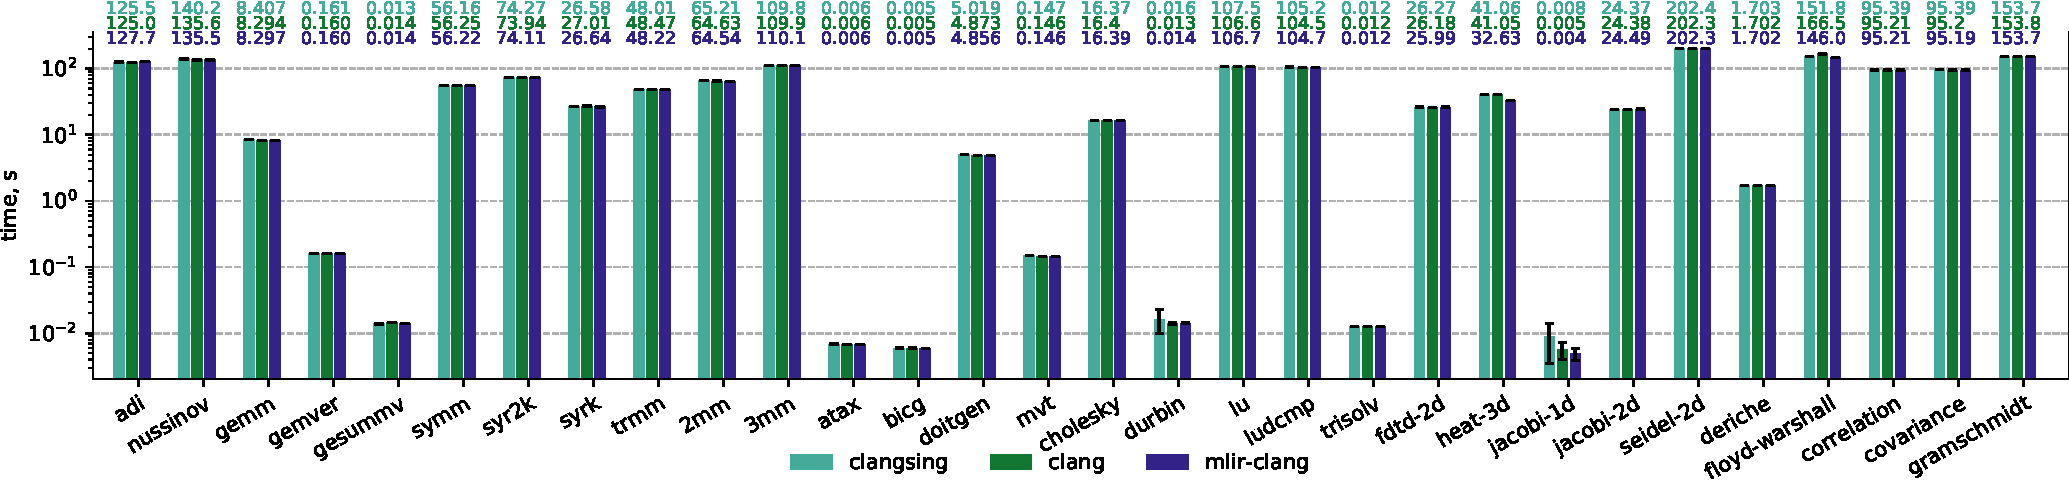
\includegraphics[width=\textwidth]{images/times.pdf}
\caption{Mean and 95\% confidence intervals (log scale) of program run time across 5 runs of Polybench in \textsc{Clang}, \textsc{ClangSing} and \textsc{MLIR-Clang} configurations, lower is better. The run times of code produced by \tool without optimization is comparable to that of Clang. No significant variation is observed between single and double optimization. Short-running \icode{jacobi-1d} shows high intra-group variation.}
\label{fig:mlir_clang}
\end{figure*}

\subsection{Compilation Flows}
\label{sub:polymer}

We compare \tool with a source-level and an IR-level optimizer (Pluto and Polly) in the following configurations:
\begin{itemize}
  \item \textsc{Pluto}: Pluto compiler auto-transformation~\cite{Bondhugula2008Pluto} using \polycc\footnote{Pluto commit \icode{dae26e77b94b2624a540c08ec7128f20cd7b7985}} with \icode{--noparallel} and \icode{--tile} flags;
  \item \textsc{PlutoPar}: Same as above but with \icode{--parallel} flag;
  \item \textsc{Polly}: Polly~\cite{grosser.ppl.2012} LLVM passes with affine scheduling and tiling, and no pattern-based optimizations~\cite{gareev_polly};
  \item \textsc{PollyPar}: Same as above with auto-parallelization;
  \item \textsc{Polygeist}: Our flow with Pluto and extra transforms;
  \item \textsc{Polygeistpar}: Same as above but with \icode{--parallel} Pluto schedule, \tool parallelization and reductions.
\end{itemize}

Running between source and LLVM IR levels, we expect \tool to benefit from both worlds, thus getting code that is on par or better than competitors.\wmnote{a bit concerned re, see email.} When using Pluto, both standalone and within \tool, we disable the emission of vectorization hints and loop unrolling to make sure both transformations are fully controlled by the LLVM optimizer, which also runs in Polly flows. We run Polly in the latest stage of Clang compilation, using \icode{--mllvm -polly} and additional flags to enable affine scheduling, tiling and parallelization as required. Polly is taken at the same LLVM commit as Clang. We disable pattern-based optimizations~\cite{gareev_polly} that are not available elsewhere.
Figures~\ref{fig:seq_speedups} and~\ref{fig:par_speedups} summarize the results for sequential and parallel flows, respectively.
%and require Polly to ignore its profitability heuristic as Pluto does not have an equivalent.  %Figures~\ref{fig:seq_speedups} and~\ref{fig:par_speedups} summarize the results for sequential and parallel flows, %respectively.
%By taking the mean absolute-value of the performance differences of all the benchmarks that have greater than 0.05 sec runtime, we find \tool has 7.76\% percentage different in runtime compared with Pluto. We will discuss the performance difference in Section~\ref{sec:perf_analysis}
%We do not compare \tool with Polly for now since Polly uses a modified version of the Pluto algorithm, making it difficult for an apple-to-apple comparison between them.

\begin{figure*}
  \centering
  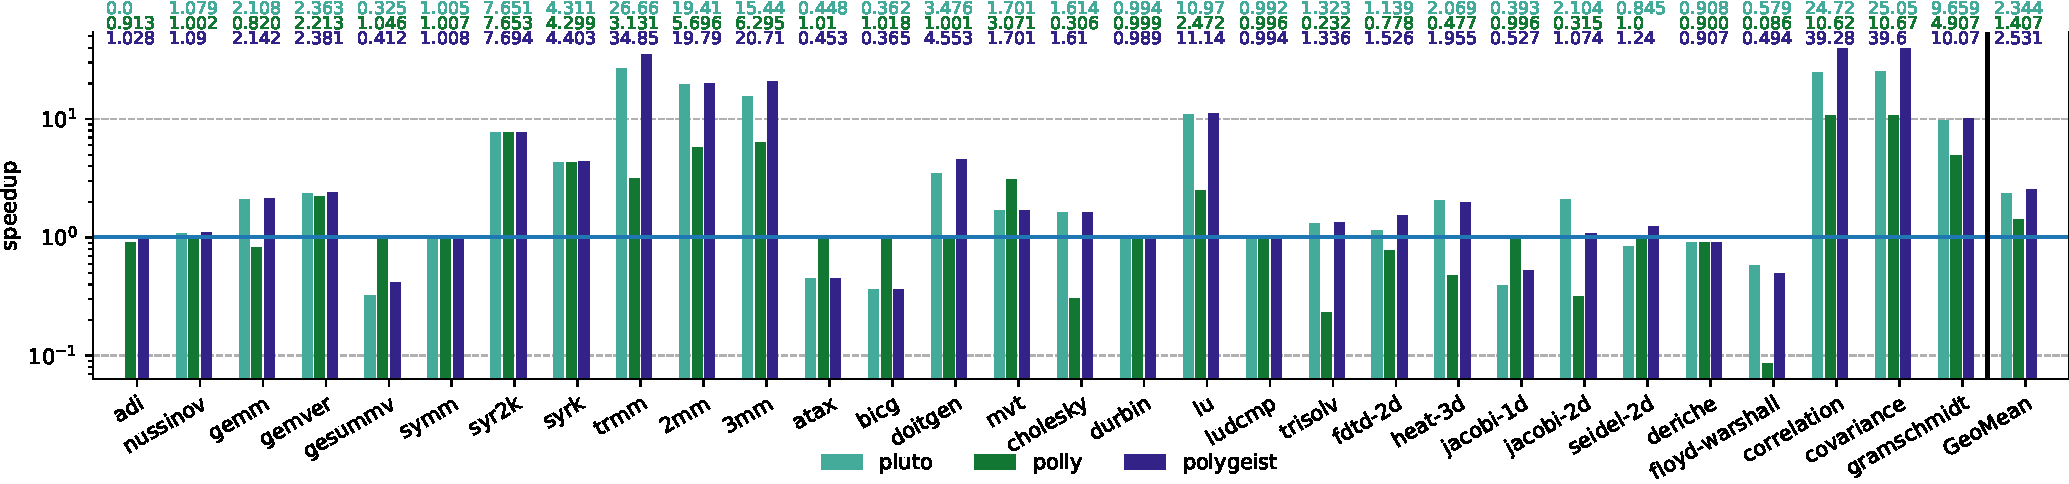
\includegraphics[width=\textwidth]{images/seq_speedups.pdf}
  \caption{Median speedup over \textsc{Clang} for sequential configurations (log scale), higher is better. \tool outperforms  (\toolseqspeedup geomean speedup) both Pluto (\plutoseqspeedup) and Polly (\pollyseqspeedup) on average. Pluto can't process \icode{adi}, which is therefore excluded from summary statistics.}
  \label{fig:seq_speedups}
\end{figure*}

\begin{figure*}
  \centering
  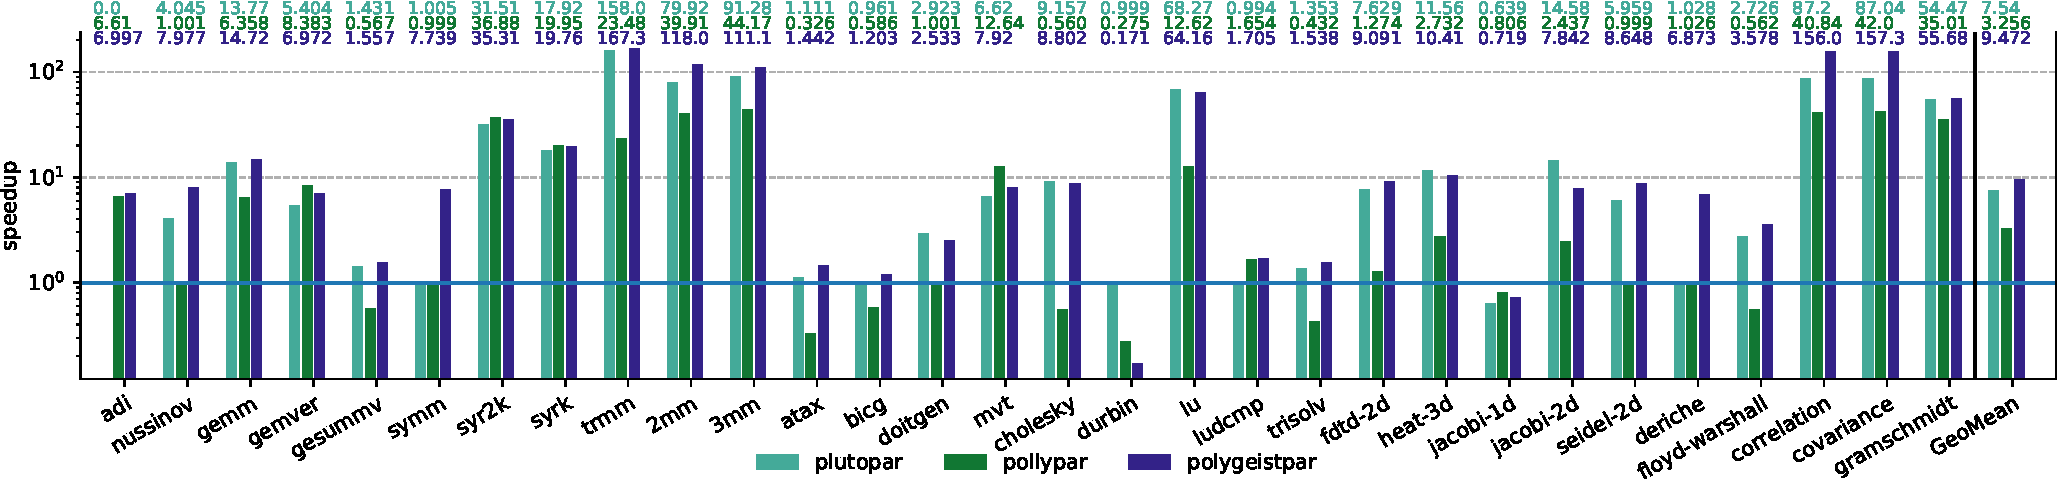
\includegraphics[width=\textwidth]{images/par_speedups.pdf}
  \caption{Median speedup over \textsc{Clang} for parallel configurations (log scale), higher is better. \tool outperforms  (\toolparspeedup geomean speedup) both Pluto (\plutoparspeedup) and Polly (\pollyparspeedup) on average. Pluto can't process \icode{adi}, which is therefore excluded from summary statistics.}
  \label{fig:par_speedups}
\end{figure*}

\section{Performance Analysis}
\subsection{Benchmarking}
The transformation of reduction loops, in particular parallelization, may result in a different order of partial result accumulation. This is not allowed under IEEE~754 semantics, but is supported by compilers with \icode{-ffast-math} option.
%, which we assume enabled.

%\az{List the benchmarks where it mattered and explain what we do to fix that.}

We found that Polybench allocation function hinders Clang/LLVM alias analysis, negatively affecting performance in, e.g., \icode{adi}. Therefore, we modified all benchmarks to use \icode{malloc} that is known to produce non-aliasing pointers.

%Finally, we found that the custom allocator used by Polybench had a nontrivial impact on the runtime of the kernel, particularly on the \icode{adi} test. This partially stems from the implementation of the allocation itself and LLVM's optimization pipeline assuming that calls to \icode{malloc} do not alias with existing allocations. To maximize the fairness of the evaluation, all flows were modified to use a standard \icode{malloc} as its memory allocation function.

\subsection{Baseline Comparison}
We did not observe a significant difference between the runtimes of \textsc{Clang} and \textsc{ClangSing} configurations, with a geometric mean of $0.43\%$ symmetric difference\footnote{Symmetric difference is computed as $2 \cdot |a - b| / (a + b)$.} across benchmarks.\wmnote{would consider removing explanation here, see email.} Therefore, we only consider \textsc{Clang} as baseline throughout the remainder of this paper. We did not observe a significant difference between the runtimes of \textsc{Clang} and \textsc{MLIR-Clang} configurations either, with a geometric mean of $0.24\%$ symmetric difference.

We found a variation in runtimes of short-running benchmarks, in particular \icode{jacobi-1d}. This can be attributed to the interaction with the data initialization and benchmarking code, and with other OS processes. Excluding the benchmarks running in under $0.05$s (\icode{jacobi-1d}, \icode{gesummv}, \icode{atax}, \icode{bicg}) from the analysis, we obtain $0.32\%$ and $0.17\%$ geomean symmetric differences respectively for the two comparisons above. These results suggest that our flow has no unexplained (dis)advantages over the baseline.

%The only benchmark with a nontrivial performance difference between \tool and Clang is the \icode{adi} test. This gap exists for two reasons: differences in allocation, and loop reversal. Specifically, compiling Polybench with Clang results in the use of a custom allocator, whereas using \tool, this results in a \memref allocation which is lowered to a \icode{malloc}. This difference in allocation function accounts for 48\% of the gap. The remaining gap exists because LLVM can strength reduce a specific load for the IR generated by Clang but not MLIR. LLVM cannot recognize this property in a reversed loop and consequently cannot perform the optimization. A future version of LLVM should permit this optimization. 

%Throughout benchmarking, we also found various behaviors of note. \tool supports the ability to compile two source files directly by producing a single MLIR module with all of the necessary functions. This is distinct from Clang, which will produce two LLVM modules that are eventually linked together. For our current benchmarks we strive to emulate the behavior of Clang by compiling the test file with \tool (e.g., nussinov.c) and linking it with timing utility code (polybench.c) using Clang. An earlier version of our pipeline, however, compiled both the timing utility code and benchmark together with \tool directly. For almost all benchmarks, this did not make a difference. But for the floyd-warshall test, we saw an 8\% reduction in performance by using a single module. An investigation into this found that interprocedural constant propagation between the utility and benchmark code allowed for significant optimization of floyd-warshall.

%Another crucial component of generating accurate code was ensuring that the code emitted by \tool had the same LLVM DataLayout and Target as that emitted by Clang natively. \tool directly parses these and marks the MLIR appropriately when it lowers Clang AST. This is not sufficient, however, as MLIR currently will not propagate the DataLayout to the eventual LLVM. This is problematic as it will result in LLVM not performing vectorization in the same way. We modified MLIR to ensure this information is propagated successfully throughout all stages of the pipeline.

\subsection{Performance Differences in Sequential Code}\label{sec:perf_analysis}
Overall, \tool leads to larger speedups, with \toolseqspeedup geometric mean, than both Pluto (\plutoseqspeedup) and Polly (\pollyseqspeedup), although improvements are not systematic. Some difference between \tool and Polly is due to the employed polyhedral schedulers, e.g., in \icode{lu} and \icode{mvt}. \tool produces code faster tha both Pluto and Polly in \icode{2mm}, \icode{3mm} and others thanks to statement splitting, see Section~\ref{sec:splitcase}.

Given identical statements and schedules, codegen-level optimization accounts for other performance difference. \icode{seidel-2d} is the clearest example: Pluto executes $2.7\!\cdot\!10^{11}$ more integer instructions than \tool. Assuming these to be index/address computations, a mix of \icode{add} (throughput $1/2$ or $1/4$) and \icode{imul/shl} (thoughput $1$), we can expect a $\approx 59$s difference at 3GHz, consistent with experimental observations. \tool optimizes away a part of those in its post-optimization phase and emits homogeneous address computation from \memref with proper machine size type, enabling more aggressive bound analysis and simplification in the downstream compiler. Conversely, \icode{jacobi-2d} has poorer performance because \tool gives up on simplifying CLooG code, with up to 75 statement copies in 40 branches, for compiler performance reasons, as opposed to Clang that takes up to 5s to process it but results in better vectorization. Further work is necessary to address this issue by emitting vector instructions directly from \tool.

%Even with the same schedule, differences in code generation may lead to performance differences. More specifically, the exact shape of domain relations fed to CLooG (e.g., the inclusion of constraints on parameters into the \emph{domain}) significantly changes the final AST. This can be addressed through a finer-grain control over the AST generation process~\cite{grosser2015polyhedral}. Furthermore, MLIR's \icode{index} type converts to the proper machine index type, which, in conjunction with automatic simplification of affine forms in MLIR, enables a more aggressive bound analysis in the downstream compiler.

%\todo{there was a nice analysis for seidel-2d, but we need new numbers here!}
%Consider, for example, \icode{seidel-2d}. \tool produces $30\%$ faster code. Analyzing the execution with \icode{perf}, we observe that both Pluto and \tool issue $143 \cdot 10^9$ FP instructions, but Pluto issues $585 \cdot 10^9$ total instructions as opposed to $254 \cdot 10^9$ by \tool. These instructions are related to control flow and address computations. Assuming a mix of \icode{add} (throughput $1/3$) and \icode{imul} (throughput $2$), the extra $331 \cdot 10^9$ instructions can comfortably explain the performance difference of 73s when running at 3GHz ($219 \cdot 10^9$ extra cycles). This can be attributed to the \memref representation that emits homogeneous, LLVM-friendly address computations.

\subsection{Performance Differences In Parallel Code}\label{sec:parallel_perf_analysis}
Similarly to sequential code, some performance differences are due to different schedulers. For example, in \icode{cholesky} and \icode{lu}, both Pluto and \tool outperform Polly, and the remaining gap can be attributed to codegen-level differences. Conversely, in \icode{gemver} and \icode{mvt} Polly has a benefit over both Pluto and \tool. On \icode{ludcmp} and \icode{syr(2)k}, SSA-level optimizations let \tool produce code which is faster than Pluto and at least as fast as Polly. These results demonstrate that \tool indeed leverages the benefits of both the affine and SSA-based optimizations.

\tool is the only flow that obtains speedup on \icode{deriche} ($6.9\times$) and \icode{symm} ($7.7\times$). Examining the output code, we observe that only \tool manages to parallelize these two benchmarks. Considering the input code in Figure~\ref{fig:deriche}, one can observe that the \icode{i} loop reuses the \icode{ym1} variable, which is interpreted as parallelism-preventing loop-carried dependency by polyhedral schedulers. \tool performs its own parallelism analysis after promoting \icode{ym1} to an SSA register (carried by the \icode{j} loop) whose use-def range does not prevent parallelization.

\begin{figure}
  \centering
  \begin{tabular}{p{0.44\linewidth}p{0.52\linewidth}}
  {\scriptsize
  \begin{lstlisting}[language=c]
for (i=0; i<_PB_W; i++){
  ym1 = SCALAR_VAL(0.0);
  // ...
  for (j=0; j<_PB_H; j++){
    ym1 = y1[i][j];
  /*...*/ }
}
  \end{lstlisting}
  }&
  {\scriptsize
  \begin{lstlisting}[language=llvm]
%z = constant 0.0 : f64
affine.parallel %i = ... {
  affine.for %j = ...
  iter_args(%ym1=%z)->f64 {
    %0=affine.load %y1[%i,%j]
    // ...
    affine.yield %0
}}
  \end{lstlisting}
  }
  \end{tabular}
  \vspace{-2em}
  \caption{Excerpt from the \icode{deriche} benchmark. The outer loop reuses \icode{ym1} which makes it appear non-parallel to affine schedulers (left). \tool detects parallelism thanks to its mem2reg optimization, reduction-like loop-carried \icode{\%ym1} value detection and late parallelization (right).}
  \label{fig:deriche}
\end{figure}

Similarly, the \tool parallelizer identifies two benchmarks with parallel reduction loops that are not contained in other parallel loops: \icode{gramschmidt} and \icode{durbin}. \icode{gramschmidt} benefits from a $56\times$ speedup with \tool, compared to $34\times$ with Polly and $54\times$ with Pluto. \icode{durbin} sees a $6\times$ slowdown since the new parallel loop has relatively few iterations and is nested inside a sequential loop, leading to synchronization costs that outweigh the parallelism benefit. Section~\ref{sec:durbin} explores the \icode{durbin} benchmark in more detail. Polybench is a collection of codes (mostly) known to be parallel and, as such, has little need for reduction parallelization on CPU where one degree of parallelism is sufficient. When targeting inherently target architectures as GPUs, however, exploiting reduction parallelism could be vital for achieving peak performance~\cite{larsen2017strategies,reduction_drawing}.

\subsection{Case Study: Statement Splitting}\label{sec:splitcase}
We identified 5 benchmarks where the statement splitting heuristic applied: \icode{2mm}, \icode{3mm}, \icode{correlation}, \icode{covariance} and \icode{trmm}. To assess the effect of the transformation, we executed these benchmarks with statement splitting disabled, suffixed with \icode{-nosplit} in Figure~\ref{fig:split_case}. In sequential versions, \icode{2mm} is $4.1\%$ slower (3.13s vs 3.26s), but the other benchmarks see speedups of $25\%$, $50\%$, $51\%$ and $27\%$, respectively. For parallel versions, the speedups are of $36\%$, $20\%$, $44\%$, $40\%$ and $-9\%$ respectively.

Examination of polyhedral scheduler outputs demonstrates that it indeed produced the desired schedules. For example, in the \texttt{correlation} benchmark which had the statement \icode{A[i][j] += B[k][i]*B[k][j]}
%original C statement
%, split into \icode{S[k] += B[k][i]*B[k][j]} and \icode{A[i][j] += S[k]},
\tool was able to find the $(k, i, j)$ loop order after splitting.
%exploiting temporal locality for \icode{B[k][i]} and spatial locality for \icode{B[k][j]}.
Using hardware performance counters on sequential code we confirm that the overall cache miss ratio has indeed decreased by $75\%, 50\%, 20\%, 27\%,$ and $-26\%$, respectively. However, the memory traffic estimated by the number of bus cycles has \emph{increased} by $9\%$ for \icode{2mm}, and decreased by $18\%, 32\%,$ $32\%$, and $21\%$ for the other benchmarks. This metric strongly correlates with the observed performance difference in the same run ($r\!\!=\!\!0.99,  p=3\!\cdot\!10^{-11}$). This behavior is likely due to the scheduler producing a different fusion structure, e.g., not fusing outermost loops in \icode{2mm}, which also affects locality. Similar results can be observed for parallel code.  Further research is necessary to exploit the statement splitting opportunities, created by \tool, and interplay with fusion.

\begin{figure}
  \centering
  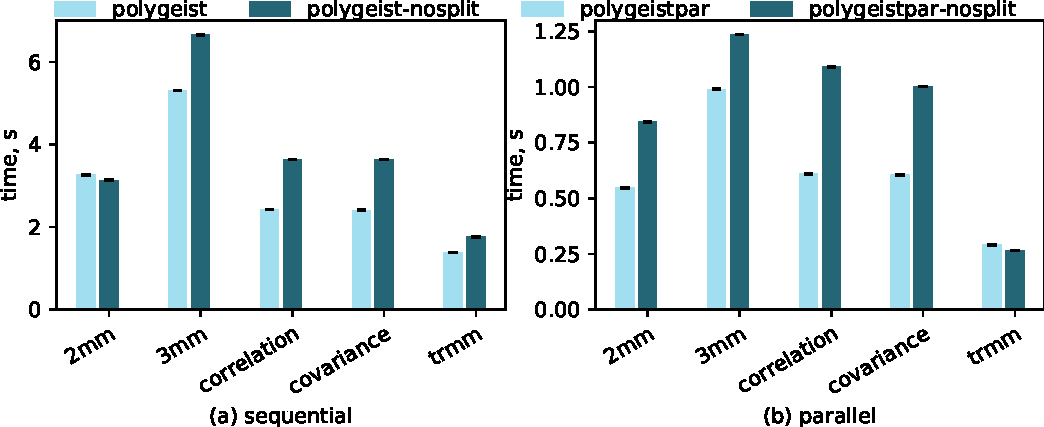
\includegraphics[width=\linewidth]{images/split.pdf}
  \caption{Mean and 95\% confidence intervals of run time across 5 runs of Polybench where statement splitting is applicable (Section~\ref{sec:stmt_splitting}), lower is better. It results in faster run time (geomean $1.28\times$ sequential, $1.39\times$ parallel speedup) except for sequential \icode{2mm} ($-4\%$) and parallel \icode{trmm} ($-9\%$).}
  \label{fig:split_case}
\end{figure}

\subsection{Case Study: Reduction Parallelization in {\tt durbin}}\label{sec:durbin}
In this benchmark, \tool uses its reduction optimization to create a parallel loop that other tools cannot. For the relatively small input run by default, $N=4000$ iterations inside another sequential loop with $N$ iterations, the overall performance decreases. We hypothesize that the cost of creating parallel threads and synchronizing them outweighs the benefit of the additional parallelism and test our hypothesis by increasing $N$. Considering the results in Figure~\ref{fig:durbin_case}, one observes that \tool starts yielding speedups ($>1$) for $N \geq 16000$ whereas Polly only does so at $N \geq 224000$, and to a much lesser extent: $6.62\times$ vs $1.01\times$. Without reduction parallelization, \tool follows the same trajectory as Polly. Pluto fails to parallelize any innermost loop and shows no speedup. This evidences in favor of our hypothesis and highlights the importance of being able to parallelize reductions.

\begin{figure}
  \centering
  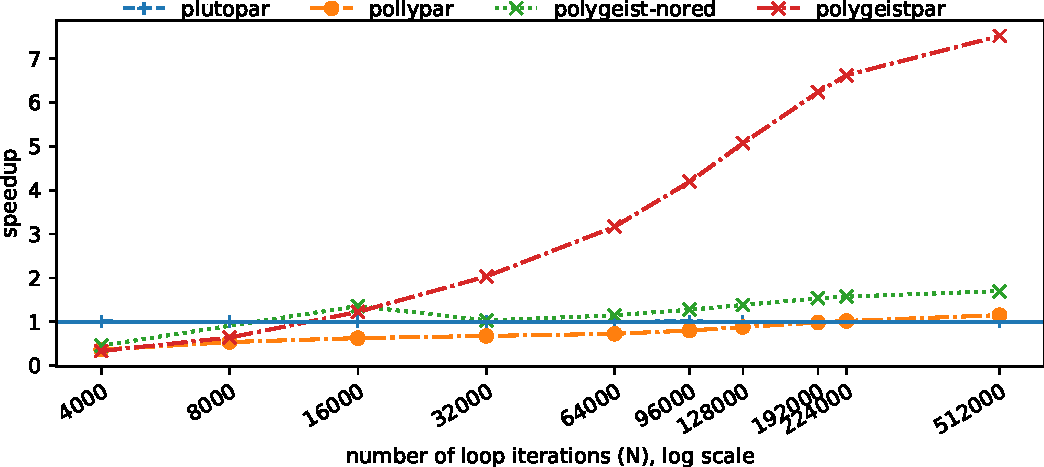
\includegraphics[width=\linewidth]{images/durbin.pdf}
  \caption{Reduction parallelization allows \textsc{{\tool}Par} to produce larger speedups in \texttt{durbin} and at smaller sizes than \textsc{PollyPar}, \textsc{{\tool}Par} without reduction support. \textsc{PlutoPar} fails to parallelize, hence no speedup.}
  \label{fig:durbin_case}
\end{figure}



\section{Related Work}


%Other proprietary compilers, such as IBM~XL~\cite{ibmxl_polyhedral} and R-Stream~\cite{rstream}, use polyhedral techniques and rely on extractor tools, but as these are proprietary little documentation is available. OpenScop~\cite{openscop} is a textual exchange format, produced by Clan among others, allowing to capture and exchange \scop.
%\lc{This OpenScop is a bit left alone.}
%\az{It is kinda the only "exchange format" out there.}


\paragraph{MLIR Frontends}

Since the adoption of MLIR under the LLVM umbrella, several frontends have been created for generating MLIR from domain-specific languages. Teckyl~\cite{teckyl} connects the productivity-oriented Tensor Comprehensions~\cite{tc} notation to MLIR's Linalg dialect. Flang---the LLVM's Fortran frontend---models Fortran-specific constructs using the FIR dialect~\cite{flang}. COMET, a domain-specific compiler for chemistry, introduces an MLIR-targeting domain-specific frontend from a tensor-based language~\cite{comet}. NPComp aims at providing the necessary infrastructure to compile numerical Python and PyTorch programs taking advantage of the MLIR infrastructure~\cite{npcomp}. PET-to-MLIR converts a subset of polyhedral C code to MLIR's Affine dialect by parsing \icode{pet}'s internal representation. In addition to currently not handling specific constructs (\icode{if}s, symbolic bounds, and external function calls), parsing \icode{pet}'s representation limits the frontend's usability as it cannot interface with non-polyhedral code such as initialization, verification, or printing routines~\cite{komisarczyk2020pet}. In contrast, \tool generates MLIR from non-polyhedral code (though not necessarily in the Affine dialect). CIRCT is a new project under the LLVM umbrella that aims to apply MLIR development methodology to the electronic design automation industry~\cite{circt}. Stripe uses MLIR Affine dialect as a substrate for loop transformations in machine learning models, including tiling and vectorization, and accepts a custom DSL as input~\cite{stripe}.

\paragraph{Compilers Leveraging Multiple Representations}

The SUIF compiler infrastructure pioneered a combined internal representation that supports higher-level transformations, including loop optimization and parallelization~\cite{wilson1994suif} and, in particular, reduction parallelization~\cite{hall1996maximizing}. \tool leverages MLIR abstractions unavailable in SUIF: regular and affine \icode{for} loops, OpenMP reduction constructs, etc. It also benefits from the SSA+regions form, which is only available as external extension in SUIF~\cite{holloway2002machine}, for IR simplification. PIPS supports loop transformations and inter-procedural optimization when targeting OpenMP~\cite{amini2011pips,amini2012par4all}. \tool differs from both by emitting machine code rather than source code, which allows it to emit parallel runtime and other directives that have no representation in the source language such as C.

\paragraph{Combining ``Classical'' and Polyhedral Flows}

Few papers have focused on combining ``classical'', mostly AST-level, and polyhedral transformations. PolyAST pioneered the approach by combining an affine scheduler with AST-level heuristics for fusion and tiling~\cite{polyast}, although similar results were demonstrated with only polyhedral transformations~\cite{spatial_scheduler}. An analogous approach was experimented in CUDA-CHiLL~\cite{zhang2016combining}. Arguably, many automated polyhedral flows perform loop fusion and/or tiling as a separate step that can be assimilated to classical transformations. Pluto~\cite{Bondhugula2008Pluto} uses several ``syntactic'' postprocessing passes to exploit spatial locality and parallelism in stencils~\cite{spatial_report}. Several tools have been proposed to drive polyhedral loop transformations with scripts using classical loop transformations such as fusion and permutation as operations, including URUK~\cite{uruk}, CHiLL~\cite{chill} and Clay~\cite{clay}. \tool differs from all of these because it preserves the results of such transformations in its IR \emph{along with} polyhedral constructs and enables interaction between different levels of abstraction.

\paragraph{Additional (Post-)Polyhedral Transformations}

Support for handling reduction loops was proposed in Polly~\cite{polly_reduction}, but the code generation is not implemented. At the syntactic level, reduction support was added to PET via manual annotation with \textsc{Pencil} directives~\cite{reduction_drawing}. R-Stream reportedly uses a variant of statement splitting to affect scheduler's behavior and optimize memory consumption~\cite{rstream}. \textsc{PolySIMD} uses variable renaming around \textsc{PPCG} polyhedral flow to improve vectorization~\cite{chatarasi2018unified}. \tool automates these leveraging both SSA and polyhedral information.

%\wmnote{I feel like this needs restructure to more conclusively say why polyhedral important, and why lacking more directly, will attempt a stab at in a bit....Future me: deciding to wait til after we chat/have a conclusive idea of what the story is overall before trying to do a pass over}
%\az{We could start with MLIR rather than polyhedral, it may be more catchy for the audience.}
%\wmnote{yeah I think that may be wise, though I guess for me generally the more catchy thing would be explaining a problem in existing flows, partial soltns (e.g. polly/pluto), and then a 10s intro to what we are.}
%\rz{Maybe it would be better to emphasize that we are focusing on polyhedral compilation flow (which is roughly the sentence ``The process of \dots'') instead of the polyhedral model in the beginning? My personal understanding of Polygeist is: the challenge in existing flows is the gap between the pipeline - program -> polyhedra -> program, and Polygeist tries to use MLIR to fill them (program -> MLIR -> polyhedra -> MLIR -> program). Putting MLIR to the start might be a bit distracted IMO.}

%The polyhedral model has remained on the cutting edge of research into compiler optimizations for several decades~\cite{feautrier2011polyhedron}.
%It provides deep loop analysis and restructuring capabilities by transforming the input program into a mathematical abstraction based on integer sets and binary relations, reasoning on this abstraction and generating the new, optimized code.
%The process of transforming the program from the representations commonly used in production compilers such as LLVM intermediate representation (IR)~\cite{llvm} or syntax tree is non-trivial~\cite{grosser.ppl.2012,pop2006graphite}, and the inverse process is even more complex~\cite{cloog,razanajato2017splitting,grosser2015polyhedral}.
%This process, together with high algorithmic complexity of the underlying transformation mechanism, has led to the polyhedral optimization being rather poorly adopted by compilers beyond research.

%MLIR is a new compiler infrastructure proposed and developed in the scope of the LLVM project~\cite{mlir}.
%One of its design goals is to provide a production-grade infrastructure that simplifies the expression of advanced compiler optimization, particularly those that require casting the input program into an additional, higher-level abstraction.
%MLIR has always considered the polyhedral representation as a first-class citizen in its infrastructure~\cite{mlir_rationale} and attempts to address the complexity and comprehensibility issues of the polyhedral model by designing and implementing all relevant algorithms from scratch. It uses a simplified representation that updates the code after each transformation instead of relying on a monolithic code generation mechanism~\cite{mlir_simplified_polyhedral}.
%\rz{Just feel that this paragraph is a bit disconnected from the previous one. We just show that the two problems of polyhedral compilation (the transformation process and algorithmic complexity), maybe after it we could directly dive into what we think is the best solution for the process problem (we don't care about poly algo), and then we can lead MLIR in.}

%The design of MLIR's affine representation~\cite{mlir_affine} makes it challenging to directly apply existing polyhedral tools, which are often based on \icode{isl}~\cite{isl} or \icode{Polylib}~\cite{polylib} and designed for C source-to-source transformation~\cite{Bondhugula2008Pluto,ppcg}. MLIR also does not include an automated polyhedral scheduler. Moreover, no benchmarks relevant for polyhedral optimization are available in MLIR. At the same time, MLIR's unique representation that combines structured region-based control flow with SSA form offers unique opportunities for combining ``classical'' SSA-based and polyhedral compiler optimizations.

%We propose \tool as a platform to connect MLIR with existing polyhedral optimizers, contributing several new techniques. First, we create a \icode{Clang}-based C and C++ MLIR frontend capable of identifying static control parts of the program (\scop) to produce the Affine dialect~\cite{mlir_affine}\rz{Should we explain what is dialect?} along with other ``standard'' MLIR dialects. Second, we implement a bi-directional conversion between the MLIR Affine dialect and the OpenScop format~\cite{openscop}. This enables a flow that originates in MLIR, uses existing standalone polyhedral tools, and returns to MLIR for further transformations and code generation. Finally, we propose two additional transformations, statement splitting and reduction parallelization, that leverage by \tool's IR\rz{It is not very clear what is Polygeist's IR, and maybe we should describe what are the objectives of these transformations (especially for statement splitting), e.g., to reduce run time.}. These transformations together with associated heuristics would have been challenging, if not impossible, to implement on either C or LLVM IR~\cite{polly_reduction,reduction_drawing}. We demonstrate that \tool can process the benchmarks of interest without significant overhead and that MLIR transformations compose with existing polyhedral flows. The combination of these contributions makes \tool competitive with state-of-the-art polyhedral compilers operating on LLVM~IR~\cite{grosser.ppl.2012} and on C~\cite{Bondhugula2008Pluto}.
%\rz{Maybe we can mention the name of Polly and Pluto here? People may find it more intriguing.}
%\az{Nah. Those who read until there will at least skim the rest. We mentioned tool names in the abstract. Also, MLIR is catchier than either of the tools anyway.}

% \az{I dropped the parts about benchmark comparisons and ablation studies because this is no longer the point of the paper}
% sg -wm

%\rz{I'm a bit confusedby the term extractor. To me it sounds like these tools simply transform from one source (IR/C) to polyhedral representation, but the description in this section actually mentions much about what kind of optimisation we can provide IMO}
\paragraph{Integration of Polyhedral Optimizers into Compilers}

Polyhedral optimization passes are available in production (GCC~\cite{pop2006graphite}, LLVM~\cite{grosser.ppl.2012}, IBM~XL~\cite{ibmxl_polyhedral}) and research (R-Stream~\cite{rstream}, ROSE~\cite{quinlan2000rose}) compilers. In most cases, the polyhedral abstraction must be extracted from a lower-level representation before being transformed and lowered in a dedicated code generation step~\cite{cloog,grosser2015polyhedral}. This extraction process is not guaranteed and may fail to recover high-level information available at the source level~\cite{delinearization}. Furthermore, common compiler optimizations such as LICM are known to interfere with it~\cite{delicm}. \tool maintains a sufficient amount of high-level information, in particular loop and n-D array structure, to circumvent these problems by design.

Source-to-source polyhedral compilers such as Pluto~\cite{Bondhugula2008Pluto} and \textsc{ppcg}~\cite{ppcg} operate on a C or C++ level. They lack interaction with other compiler optimizations and a global vision of the code, which prevents, e.g., constant propagation and inlining that could improve the results of polyhedral optimization. Being positioned between the AST and LLVM IR levels, \tool enables the interaction between higher- and lower-level abstractions that is otherwise reduced to compiler pragmas, i.e. mere optimization hints. Furthermore, \tool can rely on MLIR's progressive raising~\cite{mlir_raising} to target abstractions higher level than C code with less effort than polyhedral frameworks~\cite{tactics}.

%Source-level polyhedral extractor tools such as Clan~\cite{bastoul2008clan} and \icode{pet}~\cite{pet} identify parts of a C source code suitable for polyhedral optimization (commonly referred to as static-control parts, or \scop) and provide suitable APIs.

\section{Discussion}

\subsection{Limitations}
\paragraph{Frontend}
While \tool could technically accept any valid C or C++ thanks to building off Clang, it has the following limitations. Only \icode{struct}s with values of the same type or are used within specific functions (such as \texttt{FILE} within \texttt{fprintf}) are supported due to the lack of a struct-type in high-level MLIR dialects.  All functions that allocate memory must be compiled with \tool and not a C++ compiler to ensure that a \memref is emitted rather than a pointer.

\paragraph{Optimizer}
The limitations of the optimizer are inherited from those of the tools involved.
In particular, the MLIR affine value categorization results in all-or-nothing modeling, degrading any loop to non-affine if it contains even one non-affine access or a negative step. Running \tool's backend on code not generated by \tool's frontend, which reverses loops with negative steps, is limited to loops with positive indices. Finally, MLIR does not yet provide extensive support for non-convex sets (typically expressed as unions). Work is ongoing within MLIR to address such issues.

\paragraph{Experiments}
While our experiments clearly demonstrate the benefits of the techniques implemented in \tool --- statement splitting and late (reduction) parallelization --- non-negligible effects are due to scheduler difference: Pluto in \tool and \icode{isl} in Polly. The version of Polly using Pluto\footnote{\url{http://pluto-compiler.sourceforge.net/\#libpluto}} is not compatible with modern LLVM necessary to leverage MLIR. Connecting \icode{isl} scheduler to \tool may have yielded results closer to Polly, but still not comparable more directly because of the interplay between \scop detection, statement formation and affine scheduling.

\subsection{Opportunities and Future Work}\label{sec:opportunites}
Connecting MLIR to existing polyhedral flows opens numerous avenues for compiler optimization research, connecting polyhedral and conventional SSA-based compiler transformations.
This gives polyhedral schedulers access to important analyses such as aliasing and useful information such as precise data layout and target machine description.
Arguably, this information is already leveraged by Polly, but the representational mismatch between LLVM IR and affine loops makes it difficult to exploit them efficiently.
%This abstraction gap requires complex analyses in the polyhedral optimizer such as scalar dependence removal~\cite{delicm} or array delinearization~\cite{delinearization}.
MLIR exposes similar information at a sufficiently high level to make it usable in affine transformations.

By mixing abstractions in a single module, MLIR provides finer-grain control over the entire transformation process.
An extension of \tool can, e.g., ensure loop vectorization by directly emitting vector instructions instead of relying on pragmas, which are often merely a recommendation for the compiler. The flow can also control lower-level mechanisms like prefetching or emit specialized hardware instructions.
Conversely, polyhedral analyses can guarantee downstream passes that, e.g., address computation never produces out-of-bounds accesses and other information.

% RZ: Would the following paragraph be better? Because you've mentioned how to leverage MLIR for polyhedral, maybe the next thing to describe is the other way around. The examples 
% A polyhedral transformation flow can benefit MLIR as well.
% Based on polyhedral analysis, we can ensure that the loop is vectorized by directly emitting the corresponding vector instructions instead of relying on pragmas, which are often merely a recommendation for the compiler. The flow can also control lower-level mechanisms such as prefetching or emit specialized hardware instructions.
% Similarly, polyhedral analyses can be used to guarantee to downstream passes that address computation never produces out-of-bounds addresses and other useful information.

% RZ: maybe we can move this paragraph after the 1st one, since it also tells how to do better polyhedral analysis by MLIR?
Future work is necessary on controlling statement granularity made possible by \tool. Beyond affecting affine schedules, this technique enables easy rematerialization and local transposition buffers, crucial on GPUs~\cite{gpu_transpose}, as well as software pipelining; all without having to produce C source which is known to be complex~\cite{csmith}. On the other hand, this may have an effect on the compilation time as the number of statements is an important factor in the complexity bound of the dependence analysis and scheduling algorithms.

\subsection{Alternatives}

Instead of allowing polyhedral tools to parse and generate MLIR, one could emit C (or C++) code from MLIR\footnote{\url{https://github.com/marbre/mlir-emitc}} and use C-based polyhedral tools on the C source, but this approach decreases the expressiveness of the flow. Some MLIR constructs, such as parallel reduction loops, can be directly expressed in the polyhedral model, whereas they would require a non-trivial and non-guaranteed raising step in C. Some other constructs, such as prevectorized affine memory operations, cannot be expressed in C at all. \tool enables transparent handling of such constructs in MLIR-to-MLIR flows, but we leave the details of such handling for future work.

The \tool flow can be similarly connected to other polyhedral formats, in particular \icode{isl}. We choose OpenScop for this work because it is supported by a wider variety of tools. \icode{isl} uses schedule trees~\cite{schedule_trees} to represent the initial and transformed program schedule. Schedule trees are sufficiently close to the nested-operation IR model making the conversion straightforward: ``for'' loops correspond to band nodes (one loop per band dimension), ``if'' conditionals correspond to filter nodes, function-level constants can be included into the context node. The tree structure remains the same as that of MLIR regions. The inverse conversion can be obtained using \icode{isl}'s AST generation facility~\cite{grosser2015polyhedral}.
\section{Conclusion}
We present \tool, a compilation workflow for importing existing C or C++ code into MLIR and allows polyhedral tools, such as Pluto, to optimize MLIR programs. This enables MLIR to benefit from decades of research in polyhedral compilation. We demonstrate that the code generated by \tool has comparable performance with Clang, enabling unbiased comparisons between transformations built for MLIR and existing polyhedral frameworks. 
Finally, we demonstrate the optimization opportunities enabled by \tool considering two complementary transformations: statement splitting and reduction parallelization. In both cases, \tool achieves better performance than state-of-the-art polyhedral compiler and source-to-source optimizer.

%Finally, we demonstrate the utility of our tool to perform such integration by compiling the Polybench benchmark suite into MLIR and importing Pluto %transformations to run on MLIR programs, which may already lead to some performance improvements over the existing flows thanks to better %integration with the LLVM compiler infrastructure.
\section*{Acknowledgements}

Thanks to Valentin Churavy and Charles Leiserson of MIT for thoughtful discussions about transformations within MLIR. We
are also grateful for the numerous discussions with Tobias Grosser
from the University of Edinburgh. As well as, with Albert Cohen of Google and Henk Corporaal at TU Eindhoven.

William S. Moses was supported in part by a DOE Computational Sciences Graduate Fellowship DE-SC0019323, in part by Los Alamos National Laboratories grant 531711, and in part by the United States Air Force Research Laboratory and the United States Air Force Artificial Intelligence Accelerator and was accomplished under Cooperative Agreement Number FA8750-19-2-1000. Lorenzo Chelini is partially supported by the European Commission Horizon 2020 programme through the NeMeCo grant agreement, id. 676240. Ruizhe Zhao is sponsored by UKRI (award ref 2021246) and Corerain Technologies Ltd. The support of the UK EPSRC (grant numbers EP/L016796/1, EP/N031768/1, EP/P010040/1 and EP/L00058X/1) is also gratefully acknowledged.

The views and conclusions contained in this document are those of the authors and should not be interpreted as representing the official policies, either expressed or implied, of the United States Air Force or the U.S. Government. The U.S. Government is authorized to reproduce and distribute reprints for Government purposes notwithstanding any copyright notation herein.


\appendix
In this artifact appendix, we describe how to build Polygeist and evaluate its performance (as well as baseline compilers) on the Polybench benchmark suite. We provide two mechanisms for artifact evaluation: a Docker container\footnote{Script available here: \url{https://github.com/wsmoses/Polygeist-Script/blob/main/Dockerfile}}, and a command-by-command description of the installation process, along with comments regarding how this may need to be modified to run on a system with hardware or software configuration that is distinct from what we used. As expected, the command description mirrors much of the content of the docker file. While a docker file is certainly more convenient and a good way of getting the compiler set up, similar changes to expectations of how many cores the system has in the evaluation will be required even with Docker.

To compile Polygeist, one must first compile several of its dependencies. We ran our experiments on an AWS c5.metal instance based on Ubuntu 20.04. We've tailored our build instructions to such a system. While many of the instructions are general and independent of machine, or OS, some steps may not be (and we describe what locations they may occur below).

\begin{small}
\begin{verbatim}
$ sudo apt update
$ sudo apt install apt-utils
$ sudo apt install tzdata build-essential \
  libtool autoconf pkg-config flex bison \
  libgmp-dev clang-9 libclang-9-dev texinfo \
  cmake ninja-build git texlive-full numactl
# Change default compilers to make Pluto happy
$ sudo update-alternatives --install \
  /usr/bin/llvm-config llvm-config \
  /usr/bin/llvm-config-9 100
$ sudo update-alternatives --install \
  /usr/bin/FileCheck FileCheck-9 \
  /usr/bin/FileCheck 100
$ sudo update-alternatives --install \
  /usr/bin/clang clang \
  /usr/bin/clang-9 100
$ sudo update-alternatives --install \
  /usr/bin/clang++ clang++ \
  /usr/bin/clang++-9 100
\end{verbatim}
\end{small}

\noindent To begin, let us download a utility repository, which will contain several scripts and other files useful for compilation and benchmarking:

\begin{small}
\begin{verbatim}
$ cd 
$ git clone \
  https://github.com/wsmoses/Polygeist-Script\
  scripts
\end{verbatim}
\end{small}

\noindent One can now compile and build Pluto as shown below:

\begin{small}
\begin{verbatim}
$ cd 
$ git clone \
  https://github.com/bondhugula/pluto
$ cd pluto/
$ git checkout e5a039096547e0a3d34686295c
$ git submodule init
$ git submodule update
$ ./autogen.sh
$ ./configure
$ make -j`nproc`
\end{verbatim}
\end{small}

\noindent Next one can build LLVM, MLIR, and the frontend by performing the following:

\begin{small}
\begin{verbatim}
$ cd
$ git clone -b main-042621 --single-branch \
   https://github.com/wsmoses/Polygeist \
   mlir-clang
$ cd mlir-clang/
$ mkdir build
$ cd build/
$ cmake -G Ninja ../llvm \
 -DLLVM_ENABLE_PROJECTS="mlir;
                         polly;clang;openmp" \
 -DLLVM_BUILD_EXAMPLES=ON \
 -DLLVM_TARGETS_TO_BUILD="host" \
 -DCMAKE_BUILD_TYPE=Release \
 -DLLVM_ENABLE_ASSERTIONS=ON  
$ ninja
\end{verbatim}
\end{small}

\noindent From here, we need to modify \verb|omp.h| by copying the version from the \verb|scripts| repository and replacing the version we just built.\footnote{We modify omp.h to prevent a compilation error for Pluto parallel. The generated code does not include stdint.h, thus getting the error: unknown type name 'intptr\_t'}

\begin{small}
\begin{verbatim}
$ cd
$ export OMP_FILE=`find \
  $HOME/mlir-clang/build -iname omp.h`
$ cp $HOME/scripts/omp.h $OMP_FILE
\end{verbatim}
\end{small}

\noindent Let us now build the MLIR polyhedral analyses, along with the specific version of LLVM it requires. We shall begin by downloading the requisite code and building its dependencies.

\begin{small}
\begin{verbatim}
$ cd
$ git clone --recursive \
  https://github.com/kumasento/polymer -b pact
$ cd polymer/
$ cd llvm/
$ mkdir build
$ cd build/
$ cmake ../llvm \
  -DLLVM_ENABLE_PROJECTS="llvm;clang;mlir" \
  -DLLVM_TARGETS_TO_BUILD="host" \
  -DLLVM_ENABLE_ASSERTIONS=ON \
  -DCMAKE_BUILD_TYPE=Release \
  -DLLVM_INSTALL_UTILS=ON \
  -G Ninja
$ ninja -j`nproc`
$ ninja check-mlir
\end{verbatim}
\end{small}

\noindent We can now build the MLIR polyhedral analyses and export the corresponding build artifacts.

\begin{small}
\begin{verbatim}
$ cd ~/polymer
$ mkdir build
$ cd build
$ export BUILD=$PWD/../llvm/build
$ cmake .. \
  -DCMAKE_BUILD_TYPE=DEBUG \
  -DMLIR_DIR=$BUILD/lib/cmake/mlir \
  -DLLVM_DIR=$BUILD/lib/cmake/llvm \
  -DLLVM_ENABLE_ASSERTIONS=ON \
  -DLLVM_EXTERNAL_LIT=$BUILD/bin/llvm-lit \
  -G Ninja
$ ninja -j`nproc`
$ export LD_LIBRARY_PATH= \
    `pwd`/pluto/lib:$LD_LIBRARY_PATH
$ ninja check-polymer
\end{verbatim}
\end{small}

\noindent Finally, we are ready to begin benchmarking. We begin by running a script that disables turbo boost \& hyperthreading and remaining nonessential services on the machine. The script is specific to both the number of cores on the AWS instance (all cores except the non hyperthreaded cores on the first socket were disabled), as well as the image used (all nonessential services still present on the image were disabled) and thus may require modification if intending to be used on a different machine.

\begin{small}
\begin{verbatim}
$ cd ~/scripts/
$ sudo bash ./hyper.sh    
\end{verbatim}
\end{small}

\noindent We can now run the benchmarking script. The script itself has assumptions about cores and layout (setting \verb`taskset -c 1-8 numactl -i all` for example). If using a different machine, these settings may need to be tweaked as appropriate.

\begin{small}
\begin{verbatim}
cd ~/scripts/
$ cd polybench-c-4.2.1-beta/
$ ./run.sh
# Output comes through stdout
\end{verbatim}
\end{small}

\noindent The output of this script will contain the runtime of each trial, describing what compilation setting was used, as well as which benchmark was run.

\bibliographystyle{IEEEtran}
\bibliography{bibliography}

\end{document}
